\documentclass[cjk,slidestop,compress,mathserif,blue]{beamer}
%dvipdfm选项是关键,否则编译统统通不过
%beamer的颜色选项定义的是导航条和标题的颜色(即关键词structure的颜色)

%%%%%%%%%%%%%%%%仅限于XeTeX可使用的宏包%%%%%%%%%%%%%%%%%%%%%%%%%%%%
\usepackage{fontspec,xunicode,xltxtra,beamerthemesplit}
%\usepackage{beamerthemesplit}
\usepackage{handoutWithNotes}		%(讲义)在打印PPT的时候会留出给每一页做注释的部分
\usepackage{xeCJK}
\setCJKmainfont[BoldFont=黑体, ItalicFont=楷体, BoldItalicFont=仿宋]{黑体}
%\setsansfont[Mapping=tex-text]{Adobe 黑体 Std}
%如果装了Adobe Acrobat,可在font.conf中配置Adobe字体的路径以使用其中文字体
%也可直接使用系统中的中文字体如SimSun,SimHei,微软雅黑 等
%原来beamer用的字体是sans family;注意Mapping的大小写,不能写错

\usepackage{listings} 
\lstset{language=Matlab}%代码语言使用的是matlab 
\lstset{breaklines}%自动将长的代码行换行排版 
\lstset{extendedchars=false}%解决代码跨页时,章节标\dots

%%%%%%%%   确定标题和导航条结构的框架     %%%%%%%%%%%%
\usepackage{beamerthemeshadow}                       %
%\usepackage{beamerthemeclassic}%导航条色与背景色一致%
%%%%%%%%%%%%%%%%%%%%%%%%%%%%%%%%%%%%%%%%%%%%%%%%%%%%%%
\setbeamerfont{roman title}{size={}}
%\usepackage{CJK} % CJK 中文支持                                  %
\usepackage{amsmath,amsthm,amsfonts,amssymb,bm}
\usepackage{bbding}
\usepackage{mathrsfs}
\usepackage{xcolor}                                        %使用默认允许使用颜色
\usepackage{hyperref} 
\usepackage{graphicx}
\usepackage{subfigure}           %图片跨页
\usepackage{animate}		 %插入动画
\usepackage{tikz}		 %绘图工具
\usepackage{caption}
\captionsetup{font=footnotesize}

%\usepackage[version=3]{mhchem}		%化学公式
\usepackage{chemformula}
\usepackage{chemfig}		%化学公式

\usepackage{multirow}
\usepackage{makecell}		%允许单元格内换行

\usepackage[dvipdfmx]{movie15_dvipdfmx} %插入视频
%\usepackage{handoutWithNotes}		%(讲义)在打印PPT的时候会留出给每一页做注释的部分
%\pgfpagesuselayout{1 on 1 with notes landscape}[a4paper,border shrink=5mm]

%%%%%%%%%%%%%%%%%%%%%%BIBTEX 引用参考文献%%%%%%%%%%%%%%%%%%%%%%%%%%%%%%%%%%%%%%%%%%%%%%%%
%\usepackage{filecontents}
%\begin{filecontents*}{main.bib}
%@techreport{2012FracfocusChemical,
%  author = {FracFocus,},
%  howpublished = {\url{http://fracfocus.org/water-protection/drilling-usage}},
%  institution = {The Ground Water Protection Council and Interstate Oil and Gas
%  Compact Commission},
%  month = {feb},
%  title = {{Chemical Use In Hydraulic Fracturing}},
%  year = {2012}
%}
%\end{filecontents*}
%\usepackage[backend=bibtex,sorting=none]{biblatex}
%%\usepackage[backend=biber,style=authoryear]{biblatex}
%\addbibresource{main.bib} %BibTeX数据文件及位置

%\usepackage[numbers,sort&compress]{natbib} %紧密排列             %
\usepackage[sectionbib]{chapterbib}        %每章节单独参考文献   %
\usepackage{hypernat}                                                                         %
\setbeamertemplate{bibliography item}[text] %参考文献前标注[]
%\usepackage[dvipdfm,bookmarksopen=true,pdfstartview=FitH,CJKbookmarks]{hyperref}		%
\hypersetup{bookmarksnumbered,colorlinks,linkcolor=brown,citecolor=blue,urlcolor=red}         %
%参考文献含有超链接引用时需要下列宏包,注意与natbib有冲突        %
%\usepackage[dvipdfm]{hyperref}                                  %
%\usepackage{hypernat}                                           %
\newcommand{\upcite}[1]{\hspace{0ex}\textsuperscript{\cite{#1}}} %

%\usepackage{marvosym} %插入各种符号

%\useoutertheme{smoothbars}
\useinnertheme[shadow=true]{rounded}
\usetheme{Berkeley}                                          %主题式样
%\usetheme{Luebeck}

\usecolortheme{lily}                                        %颜色主题式样

\usefonttheme{professionalfonts}                           %字体主题样式宏包

%\beamertemplatetransparentcoveredhigh                      %使所有被隐藏的文本高度透明
\beamertemplatetransparentcovereddynamicmedium             %使所有被隐藏的文本完全透明,动态,动态的范围很小
\mode<presentation>
%\beamersetaveragebackground{gray}                          %设置背景颜色(单一色) 
\beamertemplateshadingbackground{green!10}{red!5}         %设置背景颜色(渐变色)

%i放置单位logo
%\logo{
\includegraphics[width=1.6cm,height=0.35cm]{Figures/BCC_logo-1.png}}	%简单设置logo

%\pgfdeclareimage[width=3.5cm]{logoname}{Figures/BCC_logo-1.png}		%logo置于左侧微调
%\logo{\pgfuseimage{logoname}{\vspace{0.2cm}\hspace*{-2.0cm}}}

%在指定位置精确放置logo
\usepackage{tikz}
\usepackage{beamerfoils}
\usepackage{pgf}
%\logo{\pgfputat{\pgfxy(11.68,0.15)}{
\includegraphics[height=1.01cm,viewport=0 0 140 120,clip]{Figures/BCC_logo-1.png}}\pgfputat{\pgfxy(10.502,-0.218)}{
\includegraphics[height=0.369cm,viewport=140 0 540 120,clip]{Figures/BCC_logo-1.png}}}
\logo{\pgfputat{\pgfxy(11.68,0.15)}{
\includegraphics[height=0.95cm,viewport=0 0 510 360,clip]{Figures/Logo_Gainstrong.png}}\pgfputat{\pgfxy(10.333,-0.195)}{
\includegraphics[height=0.35cm,viewport=530 70 1100 218,clip]{Figures/Logo_Gainstrong.png}}}
%\logo{\pgfputat{\pgfxy(10.28,0.00)}{
\includegraphics[height=0.95cm,viewport=0 0 1100 360,clip]{Figures/Logo_Gainstrong.png}}}
%\logo{\pgfputat{\pgfxy(11.68,0.15)}{
\includegraphics[height=0.95cm,viewport=0 0 510 360,clip]{Figures/Logo_Gainstrong.png}}\pgfputat{\pgfxy(10.333,-0.195)}{
\includegraphics[height=0.35cm,viewport=530 70 1100 218,clip]{Figures/Logo_Gainstrong.png}}}
%\MyLogo{
%	\pgfputat{\pgfxy(-50,-50)}{\pgfbox[right,base]{
\includegraphics[height=1cm]{Figures/BCC_logo-1.png}}}

%logo作为背景放置
%\setbeamertemplate{background}{
%	\pgfputat{\pgfxy(6.5,-0.5)}{\pgfbox[left,top]{\pgfimage[height=1.1cm]{Figures/BCC_logo-1.png}}}}

%\logo{}									%不显示logo

\begin{document}
%\begin{CJK*}{GBK}{song}
%\begin{CJK*}{GBK}{kai}
%beamer下不能用\songyi、\zihao等命令!
%\graphicspath{Figures/}

%\renewcommand{\figurename}{\tiny\CJKfamily{hei} 图.}
\renewcommand{\figurename}{\tiny{\bf Fig}.}
%\renewcommand{\tablename}{\tiny\CJKfamily{hei} 表.}
\renewcommand{\tablename}{\tiny{\bf Tab}.}
%\renewcommand{\tablename}{\tiny\CJKfamily{hei} 表.}
%\renewcommand{\thesubfigure}{\roman{subfigure}}  %\makeatletter 子图标记罗马字母
\renewcommand{\thesubfigure}{\tiny(\alph{subfigure})}  %\makeatletter 子图标记英文字母
%\renewcommand{\thesubfigure}{}  \makeatletter %子图无标记

%%%%%%%%%%%%%%%%%%%%%%%%%%%%%%% Latex 的 tikz 绘图 %%%%%%%%%%%%%%%%%%%%%%%%%%%%%%%%%%%%%%%%%%%
%\begin{tikzpicture}
%    % 引入图片
%    \node[anchor=south west,inner sep=0] (image) at (0,0) {\includegraphics[width=0.9\textwidth]{Mycena_interrupta.jpg}};
%
%    \begin{scope}[x={(image.south east)},y={(image.north west)}]
%        % 建立相对坐标系
%        \draw[help lines,xstep=.1,ystep=.1] (0,0) grid (1,1);
%        \foreach \x in {0,1,...,9} { \node [anchor=north] at (\x/10,0) {0.\x}; }
%        \foreach \y in {0,1,...,9} { \node [anchor=east] at (0,\y/10) {0.\y}; }
%        % 作图命令
%        \draw[red, ultra thick, rounded corners] (0.62,0.65) rectangle (0.78,0.75);
%    \end{scope}
%\end{tikzpicture}
%%%%%%%%%%%%%%%%%%%%%%%%%%%%%%%%%%%%%%%%%%%%%%%%%%%%%%%%%%%%%%%%%%%%%%%%%%%%%%%%%%%%%%%%%%%%%%

%-------------------------------PPT Title-------------------------------------
\title{\rm{VASP}计算支持的磁结构预测软件\\\rm{MagGene}简介}
%-----------------------------------------------------------------------------

%----------------------------Author & Date------------------------------------
%\author[\textrm{Jun\_Jiang}]{姜\;\;骏\inst{}} %[]{} (optional, use only with lots of authors)
% - Give the names in the same order as the appear in the paper.
% - Use the \inst{?} command only if the authors have different
%   affiliation.
\institute[BCC]{\inst{}%
% \vskip -20pt 北京市计算中心}
 \vskip 45pt 格致斯创(北京)科技有限公司}
\date[\today] % (optional, should be abbreviation of conference name)
{	%{\fontsize{6.2pt}{4.2pt}\selectfont{\textcolor{blue}{E-mail:~}\url{jiangjun@bcc.ac.cn}}}
\vskip 1 pt {\fontsize{8.2pt}{6.2pt}\selectfont{%北京理工大学%报告地点
	\vskip 2 pt \textrm{2022-01-15}}}
}

% - Either use conference name or its abbreviation
% - Not really information to the audience, more for people (including
%   yourself) who are reading the slides online

\subject{}
% This is only inserted into the PDF information catalog. Can be left
% out.
\frame
{
%	\frametitle{\fontsize{9.5pt}{5.2pt}\selectfont{\textcolor{orange}{“高通量并发式材料计算算法与软件”年度检查}}}
\titlepage
}
%-----------------------------------------------------------------------------

%------------------------------------------------------------------------------列出全文 outline ---------------------------------------------------------------------------------
\section*{}
\frame[allowframebreaks]
{
  \frametitle{Outline}
%  \frametitle{\textcolor{mycolor}{\secname}}
  \tableofcontents%[current,currentsection,currentsubsection]
}
%在每个section之前列出全部Outline
%类似的在每个subsection之前列出全部Outline是\AtBeginSubsection[]
\AtBeginSection[]
{
  \frame<handout:0>%[allowframebreaks]
  {
    \frametitle{Outline}
%全部Outline中,本部分加亮
    \tableofcontents[current,currentsection]
  }
}

%------------------------------------------------------------------------------PPT main Body------------------------------------------------------------------------------------
\small
%\section{引言}
\frame
{
	\frametitle{科学研究的范式变更}
\begin{figure}[h!]
\vspace*{0.08in}
\centering
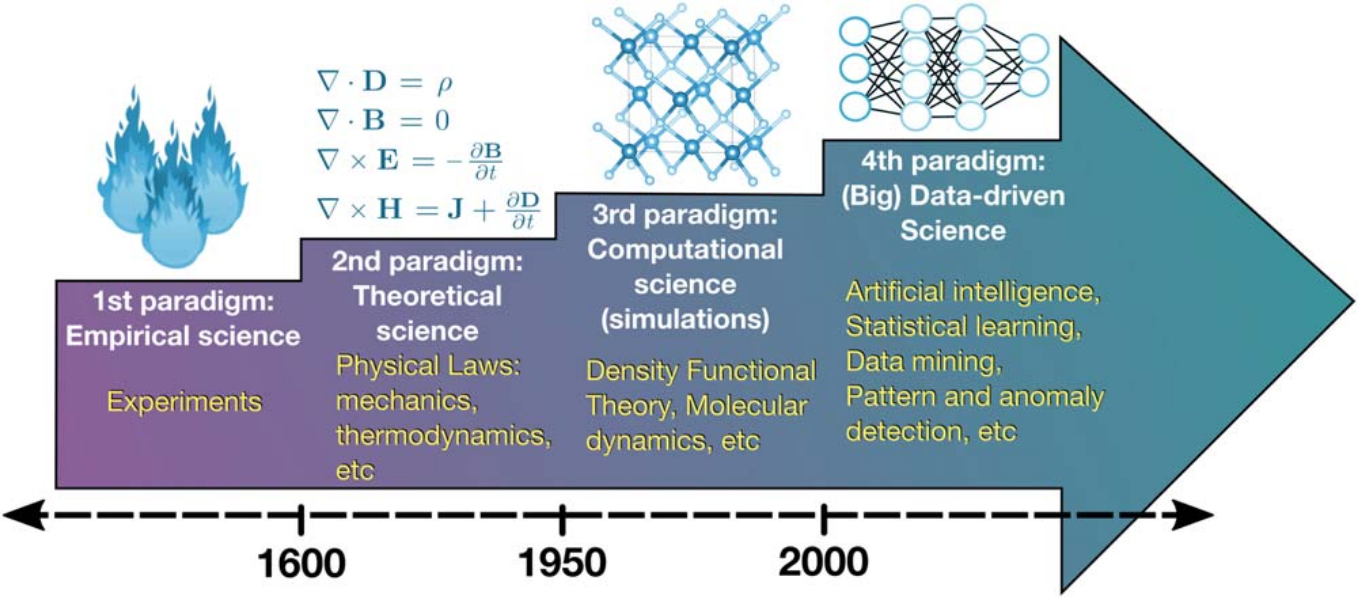
\includegraphics[width=4.15in]{Figures/Four_Model_3.png}
%\caption{\tiny \textrm{Pseudopotential for metallic sodium, based on the empty core model and screened by the Thomas-Fermi dielectric function.}}%(与文献\cite{EPJB33-47_2003}图1对比)
\label{Four_Model}
\end{figure}
}

\frame
{
	\frametitle{材料模拟的基本思想和方法}
\begin{figure}[h!]
\vspace*{-0.20in}
\centering
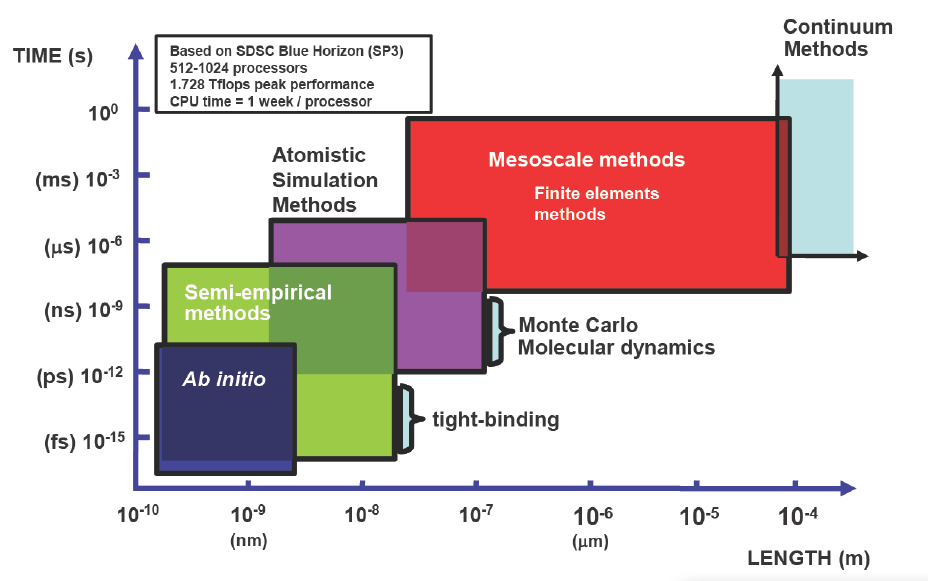
\includegraphics[height=2.20in,width=3.45in]{Figures/Multi-Scale-6.png}
\vskip 0.05pt
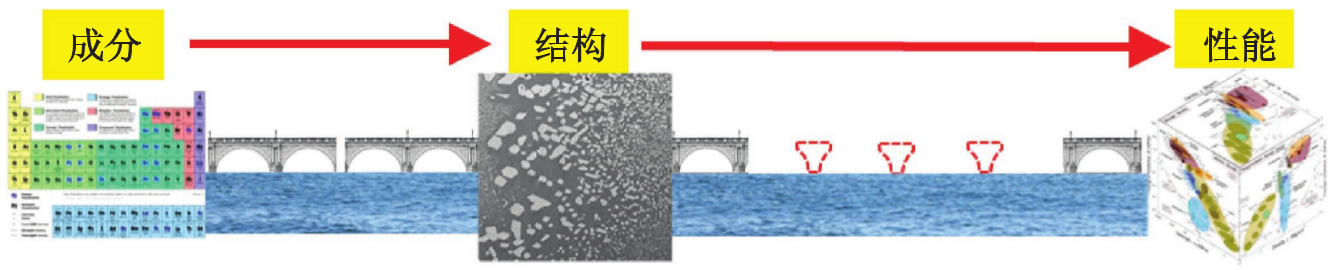
\includegraphics[height=0.80in,width=4.05in]{Figures/MGE-2.png}
%\caption{\tiny \textrm{Pseudopotential for metallic sodium, based on the empty core model and screened by the Thomas-Fermi dielectric function.}}%(与文献\cite{EPJB33-47_2003}图1对比)
\label{Multi-Scale}
\end{figure}
}

%\frame
%{
%	\frametitle{材料基因工程}
%\begin{figure}[h!]
%\vspace*{-0.18in}
%\centering
%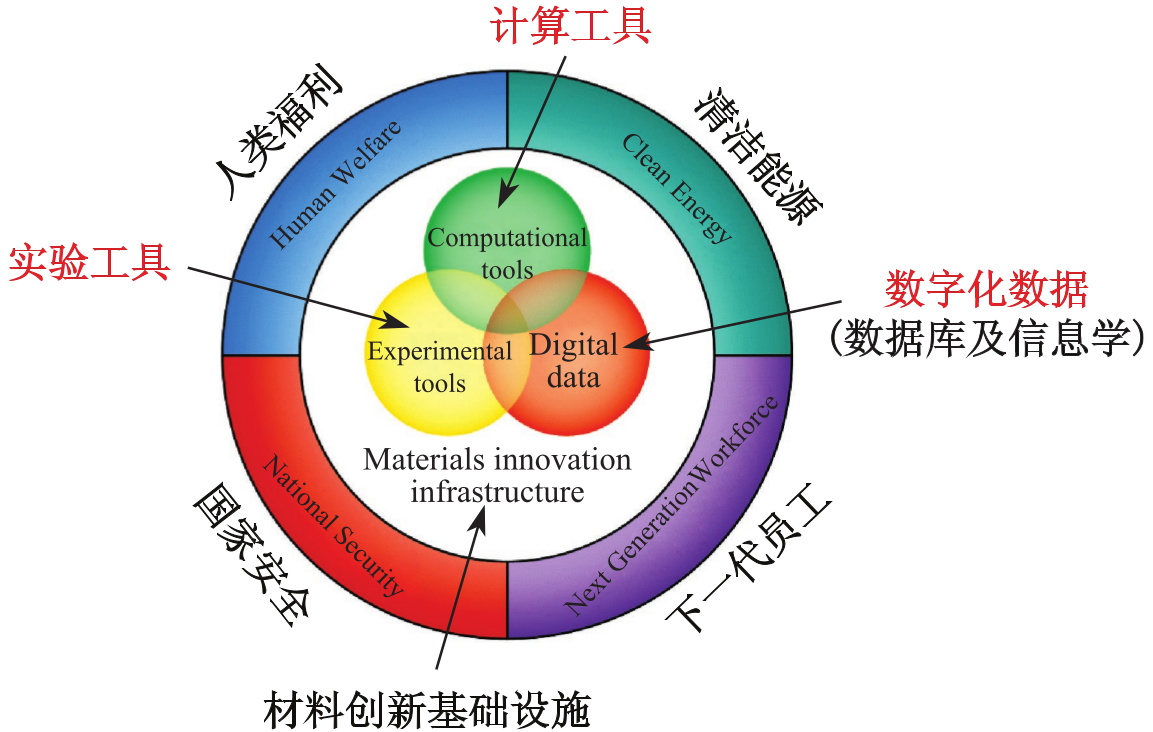
\includegraphics[height=2.55in,width=4.05in]{Figures/MGE.png}
%%\caption{\tiny \textrm{Pseudopotential for metallic sodium, based on the empty core model and screened by the Thomas-Fermi dielectric function.}}%(与文献\cite{EPJB33-47_2003}图1对比)
%%\caption{\tiny \textrm{Pseudopotential for metallic sodium, based on the empty core model and screened by the Thomas-Fermi dielectric function.}}%(与文献\cite{EPJB33-47_2003}图1对比)
%\label{MGE}
%\end{figure}
%}
\section{基本理论和\rm{VASP}软件的磁性计算}
\subsection{密度泛函理论}       %Bookmark
%\subsection{\rm{Thomas-Fermi~}模型}       %Bookmark
\frame
{
	\frametitle{\textrm{Thomas-Fermi}模型} 
	1927年,\textrm{Thomas}和\textrm{Fermi}基于均匀电子气模型上建立\textrm{Thomas-Fermi}模型,\textcolor{blue}{体系能量可用}\textcolor{red}{电子密度}\textcolor{blue}{表示}:
	\begin{itemize}
		\item 动能表达式
			$$T_{\mathrm{TF}}[\rho(\vec r)]=\dfrac3{10}(3\pi^2)^{\frac23}\int\rho^{\frac53}(\vec r)\mathrm{d}\vec r$$
		\item 外势$V_{ext}(\vec r)$下电子体系的能量泛函表达式为
			\begin{displaymath}
				\begin{aligned}
					E_{\mathrm{TF}}[\rho(\vec r)]=&\dfrac3{10}(3\pi^2)^{\frac23}\int\rho^{\frac53}(\vec r)\mathrm{d}\vec r\\
					&+\int\rho(\vec r)V_{ext}(\vec r)\mathrm{d}\vec r+\dfrac12\iint\dfrac{\rho(\vec r_1)\rho(\vec r_2)}{|\vec r_2-\vec r_1|}\mathrm{d}\vec r_1\mathrm{d}\vec r_2
				\end{aligned}
			\end{displaymath}
		\item \textrm{Thomas-Fermi}模型完全没有考虑电子的交换-相关作用
	\end{itemize}
}

\frame
{
	\frametitle{\textrm{Thomas-Fermi-Dirac}模型} 
	1930年,\textrm{Dirac}将\textrm{Thomas-Fermi}模型修正,用局域密度近似考虑电子交换作用
			\begin{displaymath}
				\begin{aligned}
					E_{\mathrm{TFD}}[\rho(\vec r)]=&\dfrac3{10}(3\pi^2)^{\frac23}\int\rho^{\frac53}(\vec r)\mathrm{d}\vec r+\int\rho(\vec r)V_{ext}(\vec r)\mathrm{d}\vec r\\
					&+\dfrac12\iint\dfrac{\rho(\vec r_1)\rho(\vec r_2)}{|\vec r_2-\vec r_1|}\mathrm{d}\vec r_1\mathrm{d}\vec r_2-\dfrac34\bigg(\dfrac3{\pi}\bigg)^{\frac13}\int\rho^{\frac43}(\vec r)\mathrm{d}\vec r
				\end{aligned}
			\end{displaymath}
			\begin{itemize}
				\item 在总电子数守恒约束条件
					$$\int\rho(\vec r)\mathrm{d}\vec r=N$$
					下,能量泛函$E_{\mathrm{TFD}}[\rho(\vec r)]$对密度$\rho(\vec r)$的变分极小获得体系的基态密度和基态能量
			\end{itemize}
}

\frame
{
	\frametitle{\textrm{Thomas-Fermi}模型}
	\begin{itemize}
		\item \textrm{Thomas-Fermi}模型用电子密度代替波函数描述问题是极大的简化,但模型过于粗糙:\\
%			\begin{enumerate}
%				\item 以均匀电子气的密度得到动能的表达式
%				\item 完全忽略电子间的交换-相关作用
%			\end{enumerate}
			不能正确描述相互作用电子体系的基本特征,如原子的壳层结构
		\item \textrm{Thomas-Fermi}模型虽不够精确,但可以通过引入修正项校正:
			\textrm{Dirac}交换泛函 $$E_X[\rho(\vec r)]=-\dfrac34\bigg(\dfrac3{\pi}\bigg)^{\frac13}\int\rho^{\frac43}(\vec r)\mathrm{d}\vec r$$
			\textrm{Wigner}相关泛函 $$E_C[\rho(\vec r)]=-0.056\int\dfrac{\rho^{\frac43}(\vec r)}{0.079+\rho^{\frac13}(\vec r)}\mathrm{d}\vec r$$
	\end{itemize}
	\textrm{Thomas-Fermi}模型为密度泛函理论\textrm{(DFT)}提供了重要的启示
}

%\subsection{密度泛函理论}       %Bookmark
\frame                               %
{
\frametitle{密度泛函理论(\textrm{DFT})} %Slide Page Title
%   \secname
与传统的量子力学方法不同,密度泛函理论的基本变量是体系的基态电子密度。%通过体系的电子密度而非波函数确定体系的基态能量。
\begin{itemize}%[+-| alert@+>]
	\item 密度泛函理论的基石:\textrm{Hohenberg-Kohn}定理\upcite{PR136-B864_1964}
\vskip 5pt
\begin{itemize}%[+-| alert@+>]
   \setlength{\itemsep}{8pt}
 \item $E[\rho]=F_{\mathrm{HK}}[\rho]+\displaystyle\int\rho(\vec{r})v(\vec{r})\textrm{d}\vec{r}$ \\
\vskip 5pt 其中$F_{\mathrm{HK}}[\rho]=\underset{\Psi\to\rho}{\mathrm{Min}}\langle\Psi[\rho]|\hat{T}+\hat{W}|\Psi[\rho]\rangle$
是普适的泛函表达式。%,指明多电子体系的基态性质与基态密度间存在一一对应关系
     \textrm{\small{第一定理表明多电子体系的性质完全由体系的基态密度决定}}
   \item 如果$\tilde\Psi\neq\Psi$,
     $E[\tilde\rho]\geqslant E[\rho_0]$\\
     \textrm{\small{第二定理指出基态总能量泛函在体系基态电子密度处取极小值}}
   \end{itemize}
%\textrm{\small{第二定理指出基态总能量泛函在体系基态电子密度处取极小值}}
\vskip 8pt
 \item 密度泛函理论的优越性:用密度($\rho$)代替波函数($\Psi$)描述体系
\vskip 5pt
 \item 密度泛函理论的困难:能量密度泛函的精确形式未知
   \end{itemize}
}

\frame                               %
{
\frametitle{密度泛函理论(\textrm{DFT})}
\textrm{Kohn-Sham}方程\upcite{PR140-A1133_1965}:无相互作用体系+交换-相关能的贡献
$$(T_S+V_{e\!f\!f})|\varphi_i\rangle=\varepsilon_i|\varphi_i\rangle,\quad i=1,\cdots,N,\cdots$$
其中$T_S=-\dfrac12\nabla^2$~~是无相互作用体系的动能
\begin{displaymath}
	\begin{aligned}
		V_{e\!f\!f}(\vec r)=&V_{ext}(\vec r)+\displaystyle\int w(\vec r,\vec r\,')\rho(\vec r\,')\mathrm{d}\vec r\,'+V_{\mathrm{XC}}[\rho]\\
=&\displaystyle\int\dfrac{\rho(\vec r\,')}{|\vec r-\vec r^{\prime}|}\mathrm{d}\vec r\,'+V_{ext}(\vec r)+V_{\mathrm{XC}}[\rho]
	\end{aligned}
\end{displaymath}
$V_{ext}(\vec r)$是电子体系与外部的电荷或磁场相互作用\\
$V_{\mathrm{XC}}[\rho]=\dfrac{\delta E_{\mathrm{XC}}}{\delta\rho(\vec r)}$称为交换-相关势
\vskip 10pt
\textrm{Kohn-Sham}方程是形式上的单粒子方程
\vskip 6pt
\textrm{Kohn-Sham}方程的实质:\\\textcolor{red}{将动能泛函的主要部分分离出来,剩余部分放在交换-相关能中}
}

\frame
{
\frametitle{交换-相关能与交换-相关势}
实际考虑交换-相关能时,会将交换-相关能表示为交换能和相关能之和:
\begin{displaymath}
	E_{\mathrm{XC}}[\rho]=E_{\mathrm{X}}[\rho]+E_{\mathrm{C}}[\rho]=\int\varepsilon_{\mathrm{X}}[\rho]\rho(\vec{r}) \textrm{d}^3\vec{r}+\int\varepsilon_{\mathrm{C}}[\rho]\rho(\vec{r}) \textrm{d}^3\vec{r}
\end{displaymath}
$\varepsilon_{\mathrm{X}}[\rho]$和$\varepsilon_{\mathrm{C}}[\rho]$可理解为单电子的交换能和相关能
\vskip 20pt
交换-相关势通过交换-相关能计算得到:~
		\begin{displaymath}
			V_{\mathrm{XC}}^{\sigma}[\rho_{\alpha},\rho_{\beta}]=\dfrac{\delta E_{\mathrm{XC}}[\rho_{\alpha},\rho_{\beta}]}{\delta\rho_{\sigma}}=\dfrac{\delta\{E_{\mathrm{X}}[\rho_{\alpha},\rho_{\beta}]+E_{\mathrm{C}}[\rho_{\alpha},\rho_{\beta}]\}}{\delta\rho_{\sigma}}
		\end{displaymath}
		\textcolor{red}{注意}:~由于$E_{\mathrm{XC}}[\rho_{\sigma}]$对$\rho_{\sigma}$是非线性的\\
		\textcolor{blue}{$V_{\mathrm{XC}}=V_{\mathrm{X}}+V_{\mathrm{C}}$和$\varepsilon_{\mathrm{XC}}=\varepsilon_{\mathrm{X}}+\varepsilon_{\mathrm{C}}$不同,不要混淆这两个量}
}
%  \beamertemplateshadingbackground{blue!10}{yellow!10}

\frame                               %
{
\frametitle{交换-相关能密度泛函}
\textcolor{blue}{密度泛函理论的核心问题}:\\
\textrm{Kohn-Sham}方程用于实际计算,必须知道$E_{\mathrm{XC}}[\rho]$或者$V_{\mathrm{XC}}[\rho]$与$\rho(\vec r)$的泛函关系
\vskip 15pt
\begin{minipage}[b]{0.59\textwidth}
 \hspace*{-15pt}
 {\fontsize{7.5pt}{6.0pt}\selectfont\begin{itemize}%[+-| alert@+>]
	 \setlength{\itemsep}{10pt}
 \item \textrm{LDA}:泛函只与密度分布的局域值有关
 \item \textrm{GGA}:泛函依赖:局域密度及其梯度
 \item $meta$-\textrm{GGA}:泛函依赖的变量还有动能密度
 \item 杂化(\textrm{hybrid})泛函:泛函与占据轨道有关
 \item 其他的交换-相关能泛函
 \item<1-> 完全非局域泛函:理想泛函,不现实
 \end{itemize}}
\end{minipage}
\hfill
\begin{minipage}[b]{0.39\textwidth}
\hspace*{-10pt}
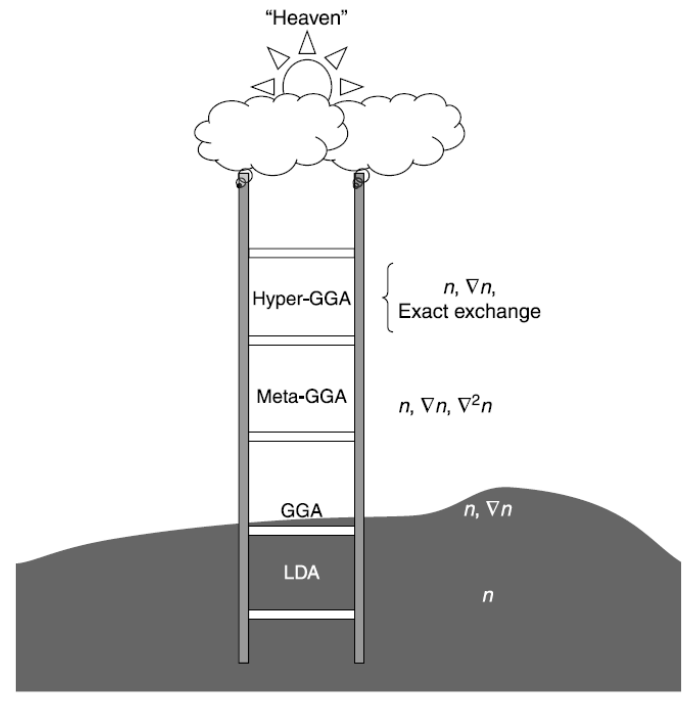
\includegraphics[height=1.7in,width=3.18in,viewport=10 5 1380 700,clip]{Figures/Jacobi-ladder.png}\\
\centering{\textcolor{red}{\textrm{\tiny Jacob's ladder}}}
\end{minipage}
% \begin{itemize}%[+-| alert@+>]
%\item 交换-相关能密度泛函
}

\frame                               %
{
	\frametitle{近似能量泛函$E_{\mathrm{XC}}[\rho]$的主要问题}
\vskip 20pt
\begin{enumerate}%[+-| alert@+>]
   \setlength{\itemsep}{10pt}
 \item  密度是整体变量:~电子自相互作用抵消不净\\%\quad\textrm{(LDA+U)}方法的校正%(\textrm{LDA+U})
	 用\textrm{DFT}计算电子数很少的体系,一般都会有较大的误差
 \item  电子相关:~简并和近简并基态的表示不合理\\
	 基态电子密度用不同的简并轨道计算时,体系能量应保持不变,但现有的近似能量泛函不具有这个性质
 \item  渐近行为:~处理弱相互作用体系的误差大\\
	 如\textrm{Van der Waals}相互作用和现有近似能量泛函本身的计算误差在同一量级
 \end{enumerate}
}

\frame
{
%	\frametitle{\textrm{DFT-SCF}}
\begin{figure}[h!]
\vspace*{-0.25in}
\centering
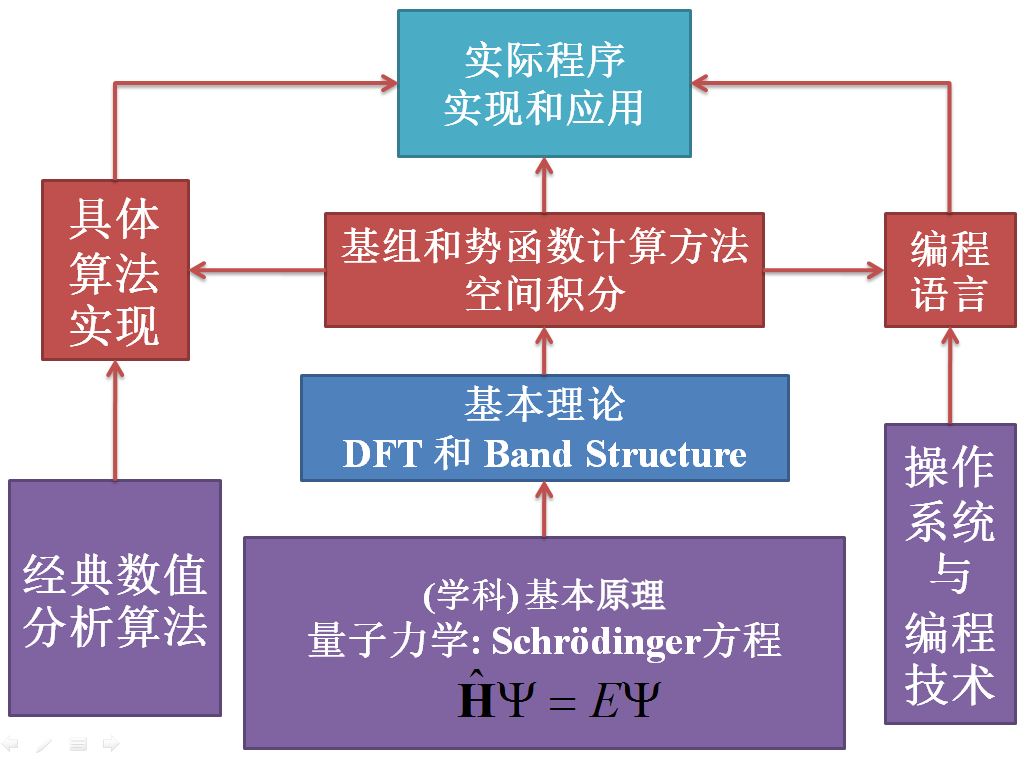
\includegraphics[height=2.80in,width=4.95in,viewport=5 3 1250 780,clip]{Figures/Method_Procedure_2.png}
%\caption{\small \textrm{Pseudopotential for metallic sodium, based on the empty core model and screened by the Thomas-Fermi dielectric function.}}%(与文献\cite{EPJB33-47_2003}图1对比)
\label{Method-Procedure}
\end{figure}
}

\frame
{
	\frametitle{\textrm{DFT-SCF}}
\begin{figure}[h!]
\centering
\vspace*{-0.25in}
\hspace*{-0.80in}
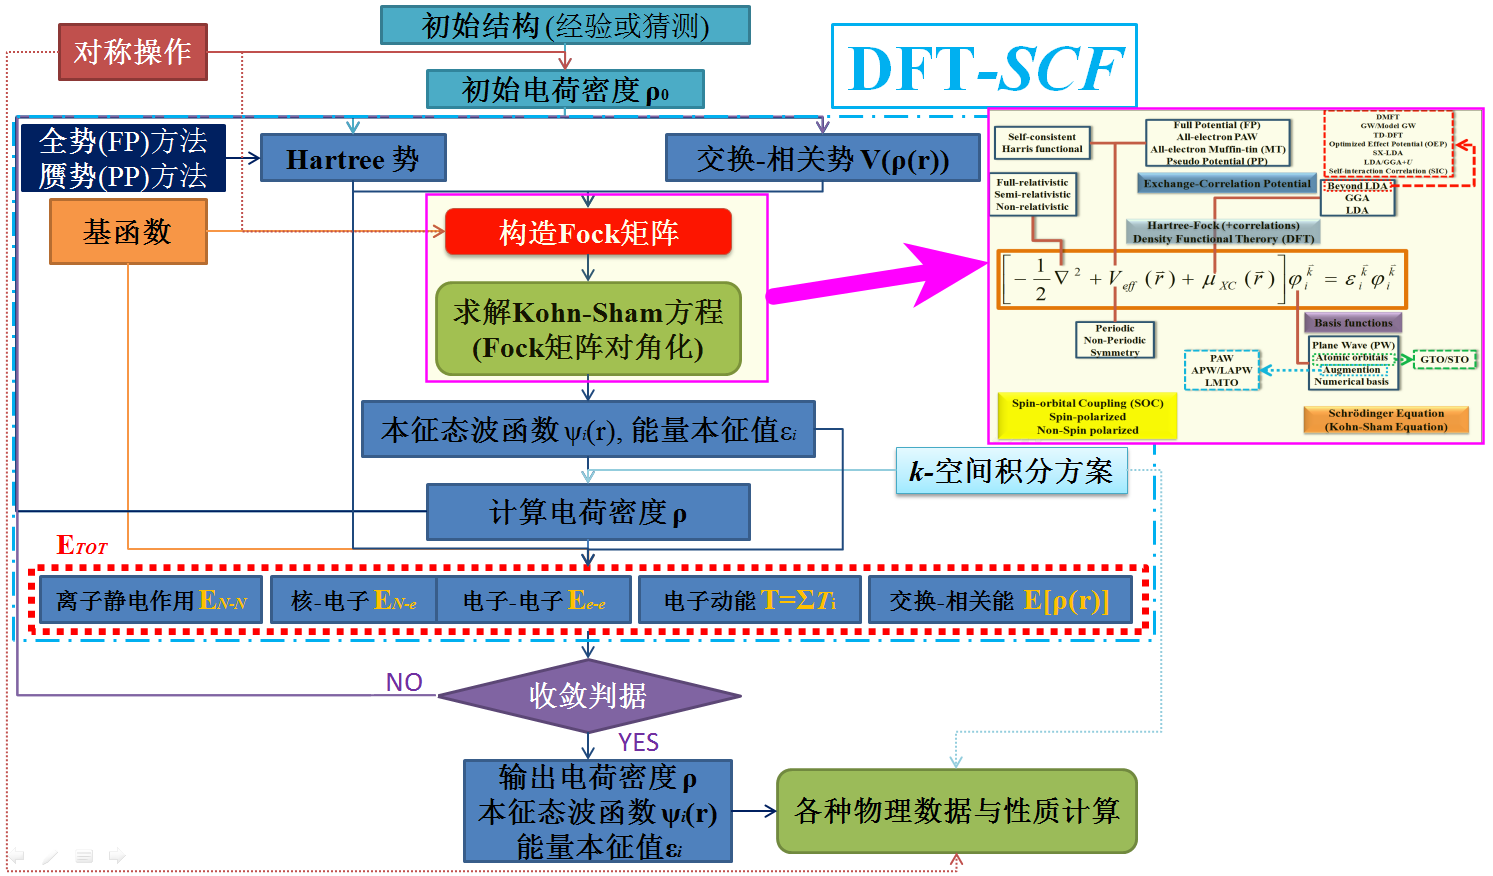
\includegraphics[height=2.80in,width=4.95in,viewport=5 3 1490 870,clip]{Figures/DFT-SCF_2.png}
%\caption{\tiny \textrm{Pseudopotential for metallic sodium, based on the empty core model and screened by the Thomas-Fermi dielectric function.}}%(与文献\cite{EPJB33-47_2003}图1对比)
\label{DFT-SCF-2}
\end{figure}
}

\subsection{\rm{VASP~}软件与\rm{PAW~}方法}
\frame
{
%	\frametitle{\textrm{PAW}原子数据集}
	\frametitle{\textrm{PAW}方法的基本思想}
\begin{figure}[h!]
\centering
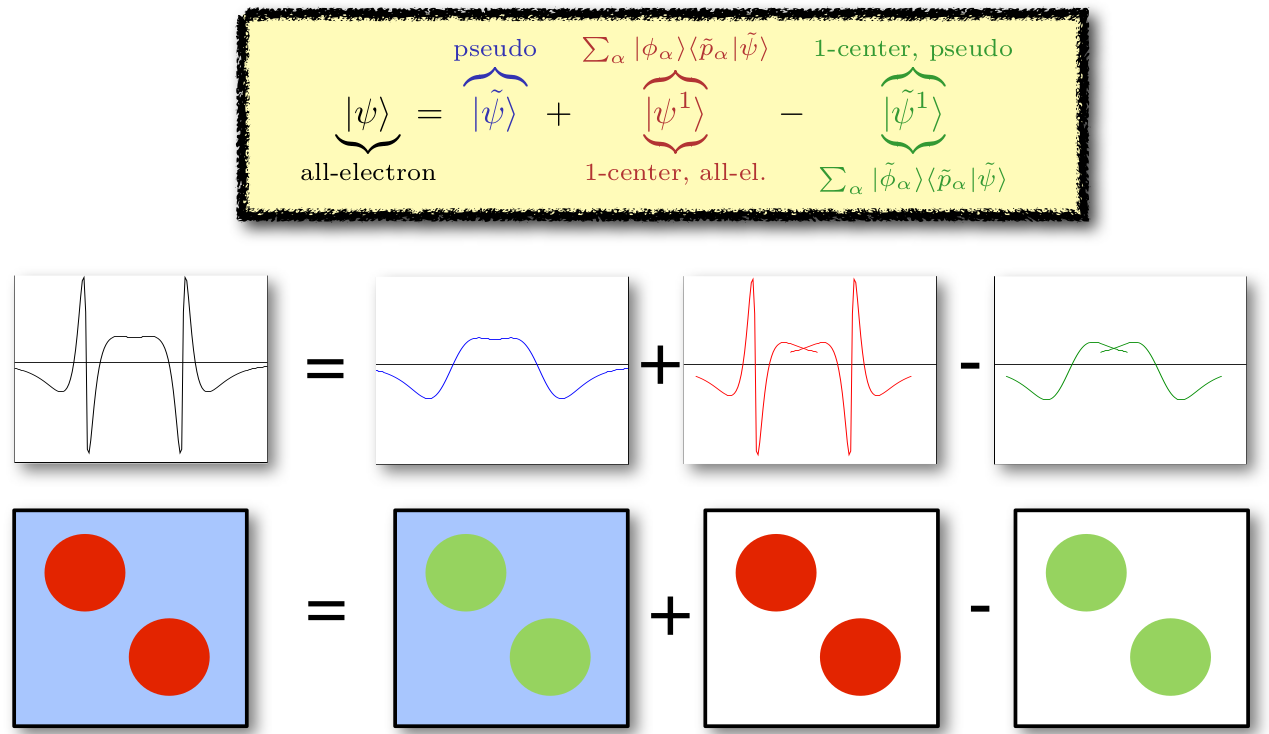
\includegraphics[height=2.3in,width=4.0in,viewport=0 0 1280 745,clip]{Figures/PAW-baseset.png}
\caption{\tiny \textrm{The Augmentation of PAW.}}%(与文献\cite{EPJB33-47_2003}图1对比)
\label{PAW_baseset}
\end{figure}
}

%\frame
%{
%	\frametitle{\textrm{PAW Augmentation}}
%\begin{figure}[h!]
%\centering
%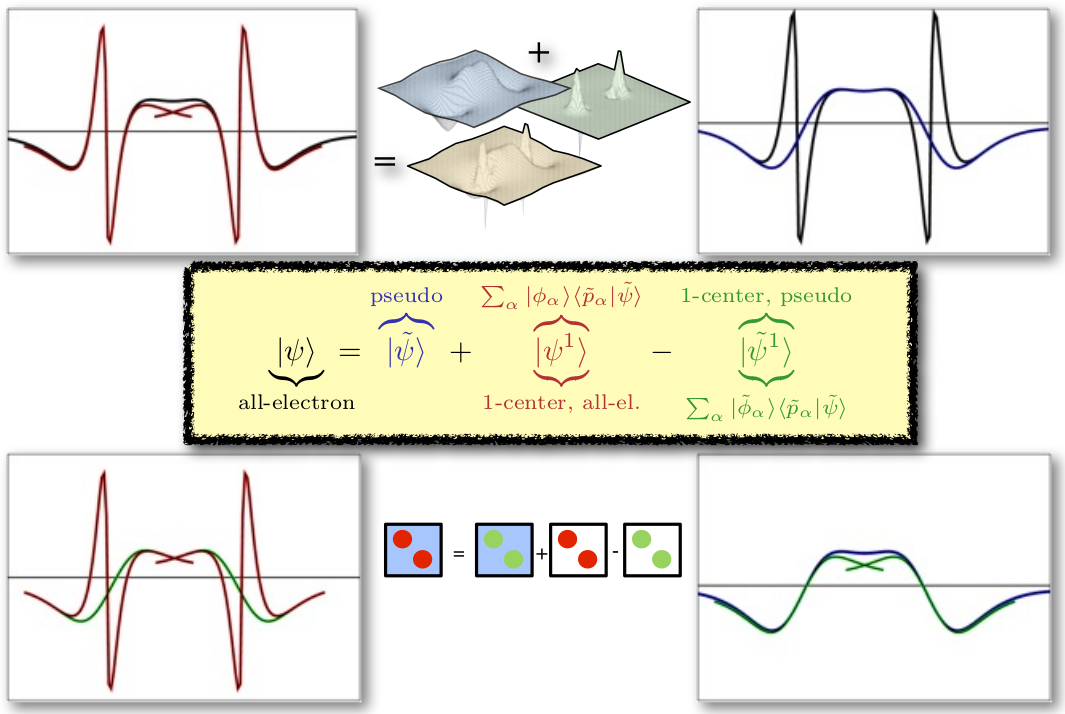
\includegraphics[height=2.3in,width=4.0in,viewport=0 0 1100 745,clip]{Figures/PAW-projector.png}
%\caption{\tiny \textrm{The projector of PAW.}}%(与文献\cite{EPJB33-47_2003}图1对比)
%\label{PAW_projector}
%\end{figure}
%}
\frame
{
	\frametitle{赝势-\textrm{PAW}方法的关系}
\begin{figure}[h!]
\centering
\vspace*{-0.20in}
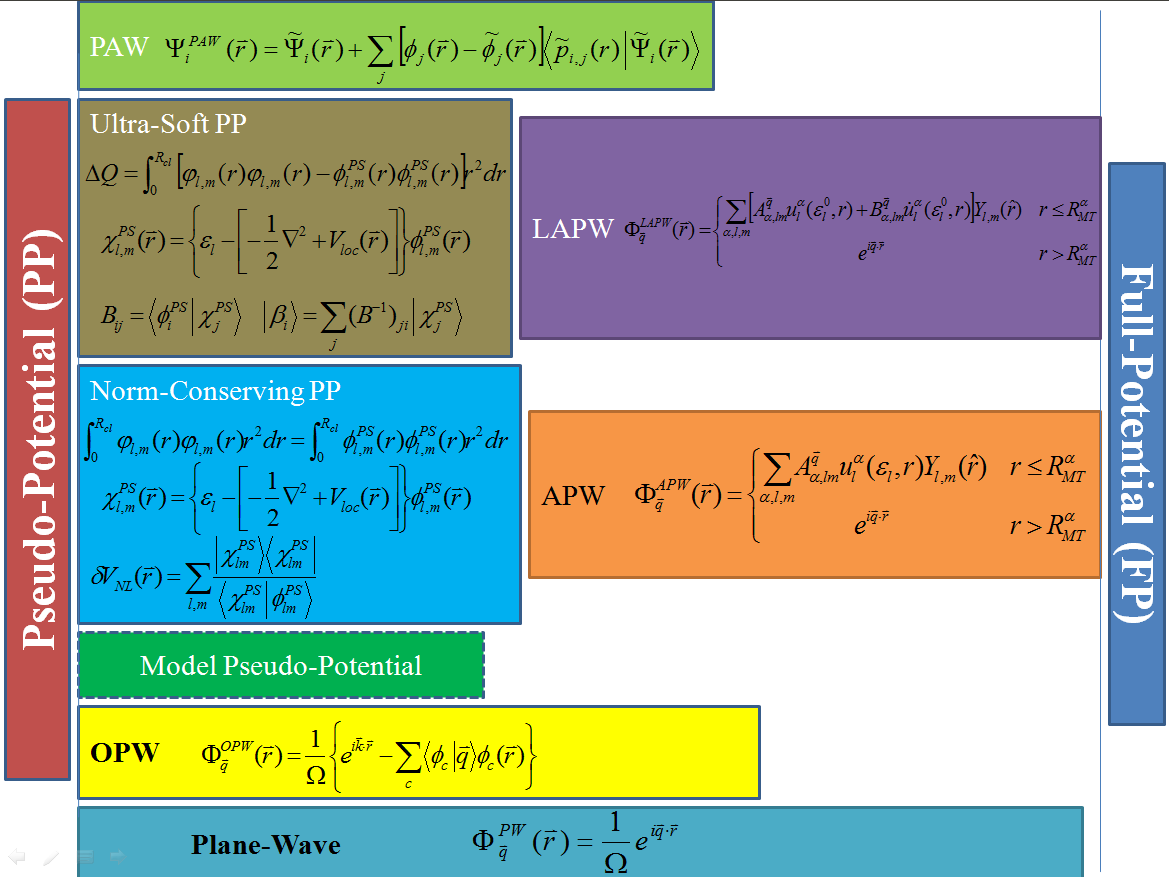
\includegraphics[height=1.90in,width=2.70in,viewport=0 0 1190 876,clip]{Figures/Pseudo-Full_Potential.png}\\
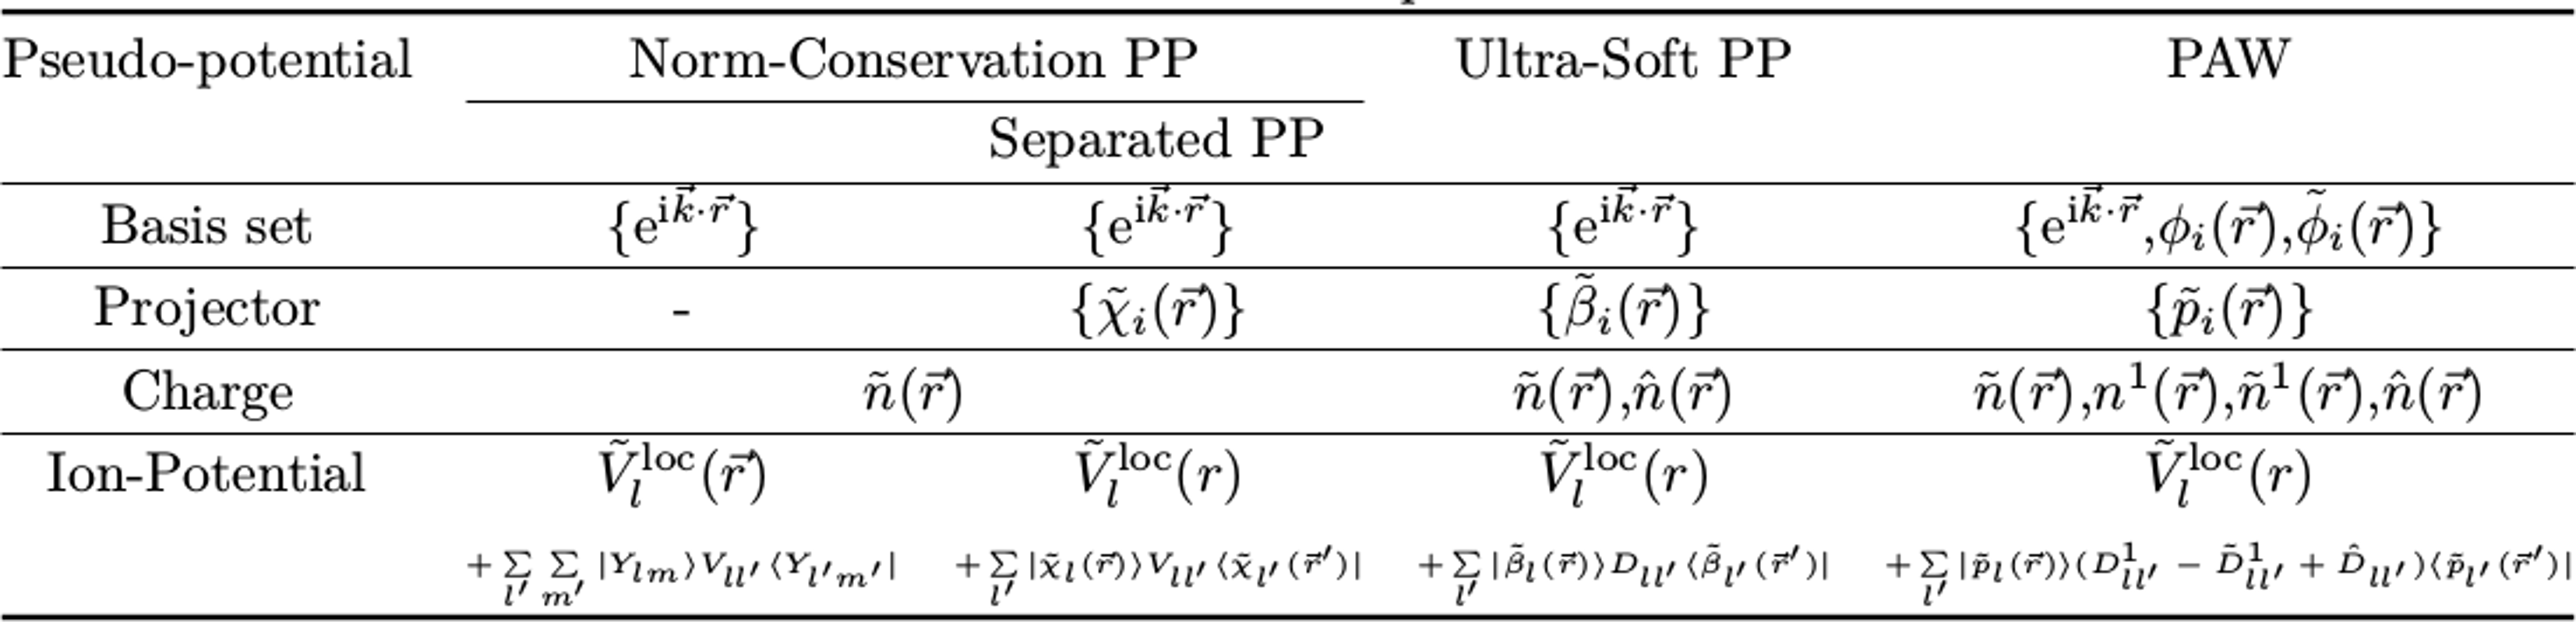
\includegraphics[height=1.0in,width=4.1in,clip]{Figures/Pseudo-Potential.png}
\caption{\tiny \textrm{The relation of Pseudo potential and PAW.}}%(与文献\cite{EPJB33-47_2003}图1对比)
\label{Pseudo_Poential}
\end{figure}
}


\frame
{
	\frametitle{\textrm{VASP}中的电荷密度的分解}
	\textrm{VASP}的开发者\textrm{G. Kresse}等明确了\textrm{PAW}方法与\textrm{USPP}方法的内在联系:
\begin{itemize}
	\item 芯层电荷与核电荷构成离子实电荷:$n_{Zc}=n_Z+n_c$
	\item 赝离子实电荷的构造$$\int_{\Omega_c}n_{Zc}(\vec r)\mathrm{d}^3\vec r=\int_{\Omega_c}\tilde n_{Zc}(\vec r)\mathrm{d}^3\vec r$$
\end{itemize}
在此基础上,\textrm{Bl\"ochl}方案中的电荷可以分解为:
\begin{displaymath}
	\begin{aligned}
		n_T=n+n_{Zc}\equiv&\underbrace{(\tilde n+\hat n+\tilde n_{Zc})}\\
				 		&\quad\qquad\tilde n_T\\
				  &+\underbrace{(n^1+\hat n+n_{Zc})}-\underbrace{(\tilde n^1+\hat n+\tilde n_{Zc})}\\
				                  &\quad\qquad n_T^1\qquad\qquad\qquad\tilde n_T^1
	\end{aligned}
\end{displaymath}
\textcolor{red}{注意}:\textrm{G. Kresse}方案中补偿电荷$\hat n$局域在每个缀加球内。
}

\frame
{
	\frametitle{总能量表达式}
	根据总能量表达式$$E=\tilde E+E^1-\tilde E^1$$其中
	\begin{displaymath}
		\begin{aligned}
			\tilde E=&\sum_nf_n\langle\tilde\Psi_n|-\frac12\nabla^2|\tilde\Psi_n\rangle+E_{\mathrm{XC}}[\tilde n+\hat n+\tilde n_c]+E_H[\tilde n+\hat n]\\
			&+\int v_H[\tilde n_{Zc}][\tilde n(\vec r)+\hat n(\vec r)]\mathrm{d}\vec r+U(\vec R,Z_{\mathrm{ion}})\\
			\tilde E^1=&\sum_{(i,j)}\rho_{ij}\langle\tilde\phi_i|-\frac12\nabla^2|\tilde\phi_j\rangle+\overline{E_{\mathrm{XC}}[\tilde n^1+\hat n+\tilde n_c]}+\overline{E_H[\tilde n^1+\hat n]}\\
			&+\int_{\Omega_r}v_H[\tilde n_{Zc}][\tilde n^1(\vec r)+\hat n(\vec r)]\mathrm{d}\vec r
		\end{aligned}
	\end{displaymath}
}

\frame
{
	\frametitle{总能量表达式}
	\begin{displaymath}
		\begin{aligned}
			E^1=&\sum_{(i,j)}\rho_{ij}\langle\phi_i|-\frac12\nabla^2|\phi_j\rangle+\overline{E_{\mathrm{XC}}[n^1+n_c]}+\overline{E_H[n^1]}\\
			&+\int_{\Omega_r}v_H[n_{Zc}]n^1(\vec r)\mathrm{d}\vec r
		\end{aligned}
	\end{displaymath}
	$v_H$是电荷密度$n$产生的静电势
	$$v_H[n](\vec r)=\int\dfrac{n(\vec r\,^{\prime})}{|\vec r-\vec r\,^{\prime}|}\mathrm{d}\vec r\,^{\prime}$$
	$E_H[n]$是对应的静电能
	$$E_H[n]=\dfrac12(n)(n)=\dfrac12\int\mathrm{d}\vec r\mathrm{d}\vec r\,^{\prime}\dfrac{n(\vec r)n(\vec r\,^{\prime})}{|\vec r-\vec r\,^{\prime}|}$$ 
	$U(\vec R,Z_{\mathrm{ion}})$\textcolor{blue}{由\textrm{Ewald}求和计算}
}

\frame
{
	\frametitle{补充电荷的构造}
	根据约束条件
	\begin{displaymath}
		\int_{\Omega_c}(n^1-\tilde n^1-\hat n)|\vec r-\vec R|^lY_{lm}^{\ast}(\widehat{\vec r-\vec R})\mathrm{d}\vec r=0
	\end{displaymath}
	定义电荷密度差
	\begin{displaymath}
		Q_{ij}(\vec r)=\phi_i^{\ast}(\vec r)\phi_j(\vec r)-\tilde\phi_i^{\ast}(\vec r)\tilde\phi_j(\vec r)
	\end{displaymath}
	电荷密度差的多极矩为
	\begin{displaymath}
		q_{ij}^L(\vec r)=\int_{\Omega_r}Q_{ij}(\vec r)|\vec r-\vec R|^lY_{lm}^{\ast}(\widehat{\vec r-\vec R})\mathrm{d}\vec r
	\end{displaymath}
	因此,补充电荷的计算为:
	\begin{displaymath}
		\begin{aligned}
			\hat n=\sum_{(i,j),L}\sum_n f_n\langle\tilde\Psi_n|\tilde p_i\rangle\langle\tilde p_j|\Psi_n\rangle\hat Q_{ij}^L(\vec r)\\
			\hat Q_{ij}^L(\vec r)=q_{ij}^Lg_l(|\vec r-\vec R|)Y_{lm}(\widehat{\vec r-\vec R})
		\end{aligned}
	\end{displaymath}
}

\frame
{
	\frametitle{重叠矩阵和\textrm{Hamiltonian~}的构造}
重叠矩阵
	\begin{displaymath}
		\langle\tilde\Psi_n|\mathbf{S}|\tilde\Psi_m\rangle=\delta_{nm}
	\end{displaymath}
	其中重叠矩阵$$S[\{\mathbf{R}\}]=1+\sum_i|\tilde p_i\rangle q_{ij}\langle\tilde p_j|$$
	而$$q_{ij}=\langle\phi_i|\phi_j\rangle-\langle\tilde\phi_i|\tilde\phi_j\rangle$$
	\textrm{Hamiltonian}的计算
	\begin{displaymath}
		H[\rho,\{\mathbf{R}\}]=-\dfrac12\nabla^2+\tilde v_{e\!f\!f}+\sum_{(i,j)}|\tilde p_i\rangle(\hat D_{ij}+D_{ij}^1-\tilde D_{ij}^1)\langle\tilde p_j|	
	\end{displaymath}
	$$\tilde v_{e\!f\!f}=v_H[\tilde n+\hat n+\tilde n_{Zc}]+v_{\mathrm{XC}}[\tilde n+\hat n+\tilde n_{Zc}]$$
}

\frame
{
	\frametitle{重叠矩阵和\textrm{Hamiltonian~}的构造}
	$$\hat D_{ij}=\dfrac{\partial\tilde E}{\partial\rho_{ij}}=\int\dfrac{\delta\tilde E}{\delta\hat n(\vec  r)}\dfrac{\partial\hat n(\vec r)}{\partial\rho_{ij}}\mathrm{d}\vec r=\sum_{L}\int\tilde v_{e\!f\!f}\hat Q_{ij}^L(\vec r)\mathrm{d}\vec r$$
	$$D_{ij}^1=\dfrac{\partial E^1}{\partial\rho_{ij}}=\langle\phi_i|-\dfrac12\nabla^2+v_{e\!f\!f}^1|\phi_j\rangle$$
	其中$$v_{e\!f\!f}^1[n^1]=v_H[n^1+n_{Zc}]+v_{\mathrm{XC}}[n^1+n_c]$$
	$$\tilde D_{ij}^1=\dfrac{\partial\tilde E^1}{\partial\rho_{ij}}=\langle\tilde\phi_i|-\dfrac12\nabla^2+\tilde v_{e\!f\!f}^1|\tilde\phi_j\rangle+\sum_L\int_{\Omega_r}\mathrm{d}\vec r\tilde v_{e\!f\!f}^1(\vec r)\hat Q_{ij}^L$$
	其中$$\tilde v_{e\!f\!f}^1[\tilde n^1]=v_H[\tilde n^1+\hat n+\tilde n_{Zc}]+v_{\mathrm{XC}}[\tilde n^1+\hat n+\tilde n_c]$$
}

\frame
{
	\frametitle{\textrm{Double counting correlations}}
	能带计算中,总能量可通过\textrm{Kohn-Sham}本征值求和扣除\textrm{Double counting}计算更方便,其中修正项
	\begin{displaymath}
		\begin{aligned}
			\tilde E_{dc}=&-E_H[\tilde n+\hat n]+E_{\mathrm{XC}}[\tilde n+\hat n+\tilde n_c]\\
			&-\int v_{\mathrm{XC}}[\tilde n+\hat n+\tilde n_c](\tilde n+\hat n)\mathrm{d}\vec r\\
			E_{dc}^1=-\overline{E_H[n^1]}&+\overline{E_{\mathrm{XC}}[n^1+n_c]}-\int_{\Omega_r}v_{\mathrm{XC}}[n^1+n_c]n^1\mathrm{d}\vec r\\
			\tilde E_{dc}^1=&-\overline{E_H[\tilde n^1+\hat n]}+\overline{E_{\mathrm{XC}}[\tilde n^1+\hat n+\tilde n_c]}\\
			&-\int v_{\mathrm{XC}}[\tilde n^1+\hat n+\tilde n_c](\tilde n^1+\hat n)\mathrm{d}\vec r
		\end{aligned}
	\end{displaymath}
	因此总能量的计算表达式是
	$$E=\sum_nf_n\langle\tilde\Psi_n|H|\tilde\Psi_n\rangle+\tilde E_{dc}+E_{dc}^1-\tilde E_{dc}^1+U(\vec R,Z_{\mathrm{ion}})$$
}

\frame
{
	\frametitle{计算流程}
\begin{figure}[h!]
	\vspace{-0.2in}
\centering
%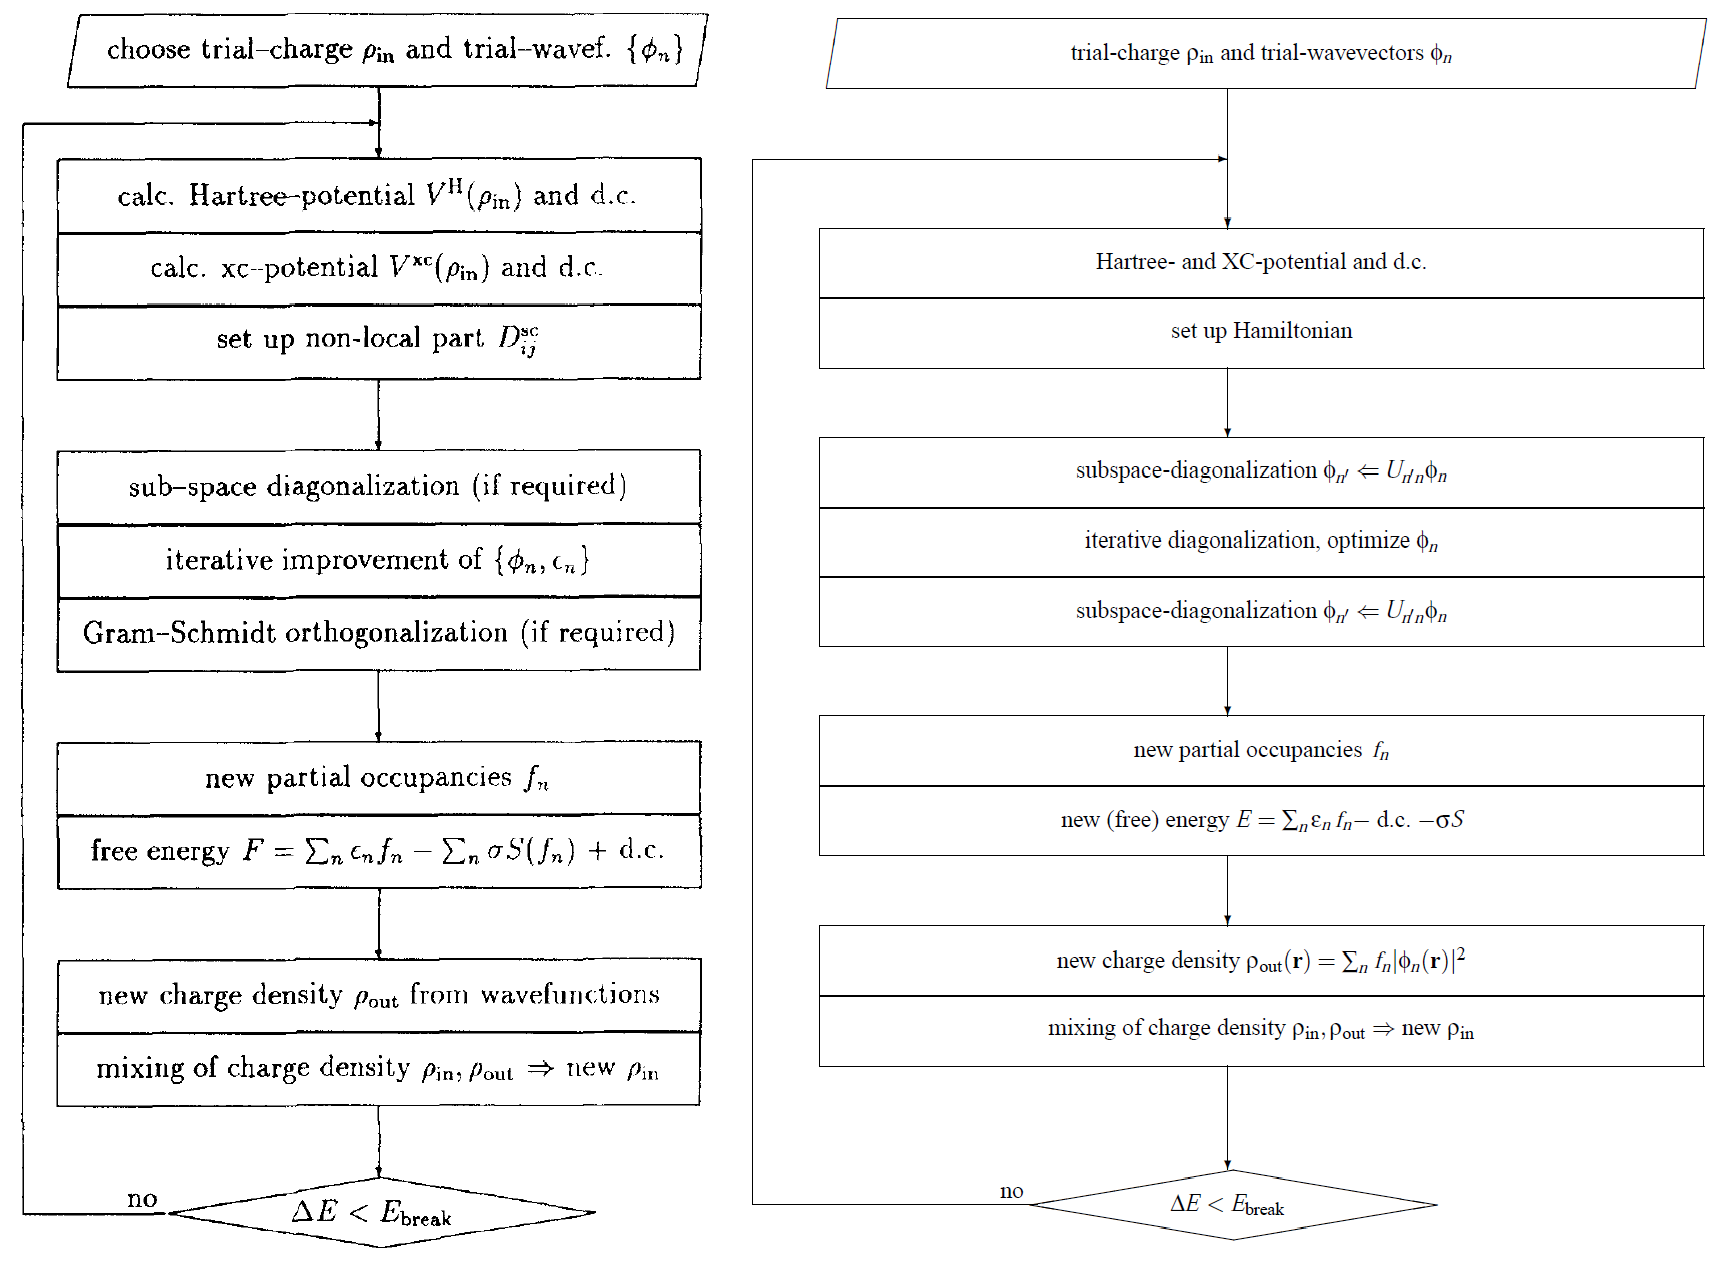
\includegraphics[height=2.7in,width=4.0in,viewport=0 0 1300 960,clip]{Figures/VASP_procedure-full.png}
%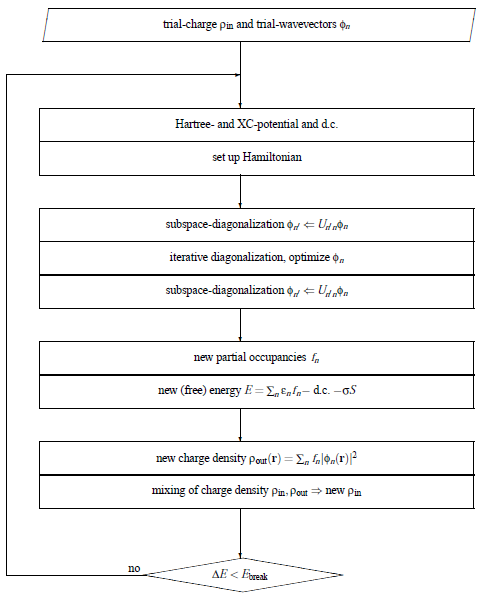
\includegraphics[height=2.1in,width=1.6in,viewport=0 0 480 630,clip]{Figures/VASP_procedure.png}
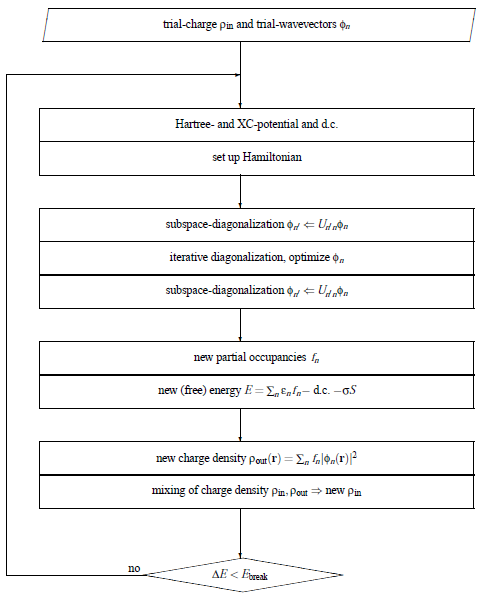
\includegraphics[height=2.1in,width=1.6in,viewport=0 0 480 630,clip]{Figures/VASP_procedure.png}
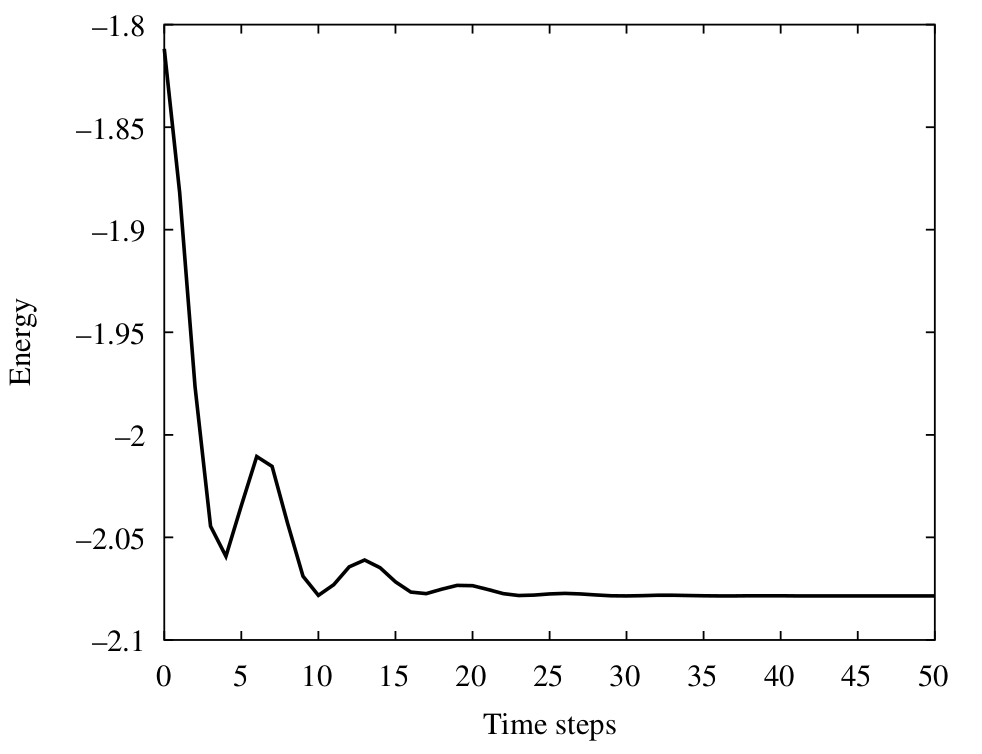
\includegraphics[height=2.1in,width=2.3in,viewport=0 0 740 600,clip]{Figures/Ab-initio-Ene.png}
\caption{\tiny \textrm{The Flow of calculation for the KS-ground states.}}%(与文献\cite{EPJB33-47_2003}图1对比)
\label{PAW_baiseset}
\end{figure} 
}

\frame
{
	\frametitle{\textrm{VASP}计算的特色}
	相比于与普通的第一原理计算软件,\textrm{VASP}很好地平衡了计算效率和精度的问题,总的来说,\textrm{VASP}主要通过这几个特色保证了计算的高效能
	\begin{itemize}
	     \item 迭代与优化算法的多样性\\
		     本质上电荷密度迭代 \textrm{\&\&} 体系总能量优化是相同的优化问题,采用了类似的算法\upcite{CMS6-15_1996,PRB54-11169_1996}:\\
			\textcolor{blue}{\textrm{Pseudo-Newton、Conjugate-Gradient、Broyden~mix、damping-factor、RMM-DIIS}}
	     \item 尽可能采用局域基(原子轨道基)函数:~\\
		     \textcolor{blue}{\textrm{LREAL}}=\textcolor{red}{\textrm{.TRUE.}}\\
			优化的投影函数也尽可能在实空间表示
	     \item \textrm{PAW}原子数据集:\textcolor{blue}{优异的赝势}\upcite{PRB59-1758_1999}
	\end{itemize}
}

\frame
{
	\frametitle{双网格技术}
\begin{figure}[h!]
	\vspace{-0.2in}
\centering
%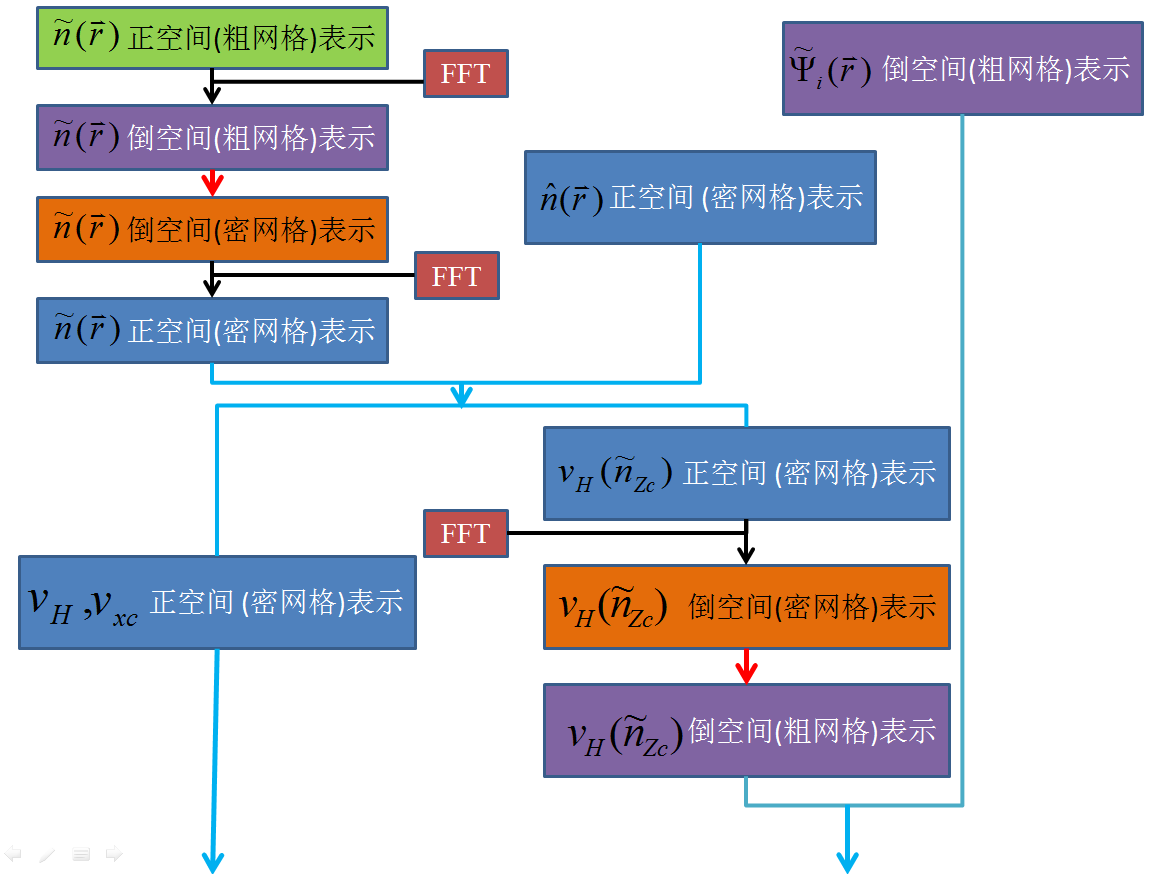
\includegraphics[height=2.7in,width=4.0in,viewport=0 0 1180 875,clip]{Figures/dual_grid.png}
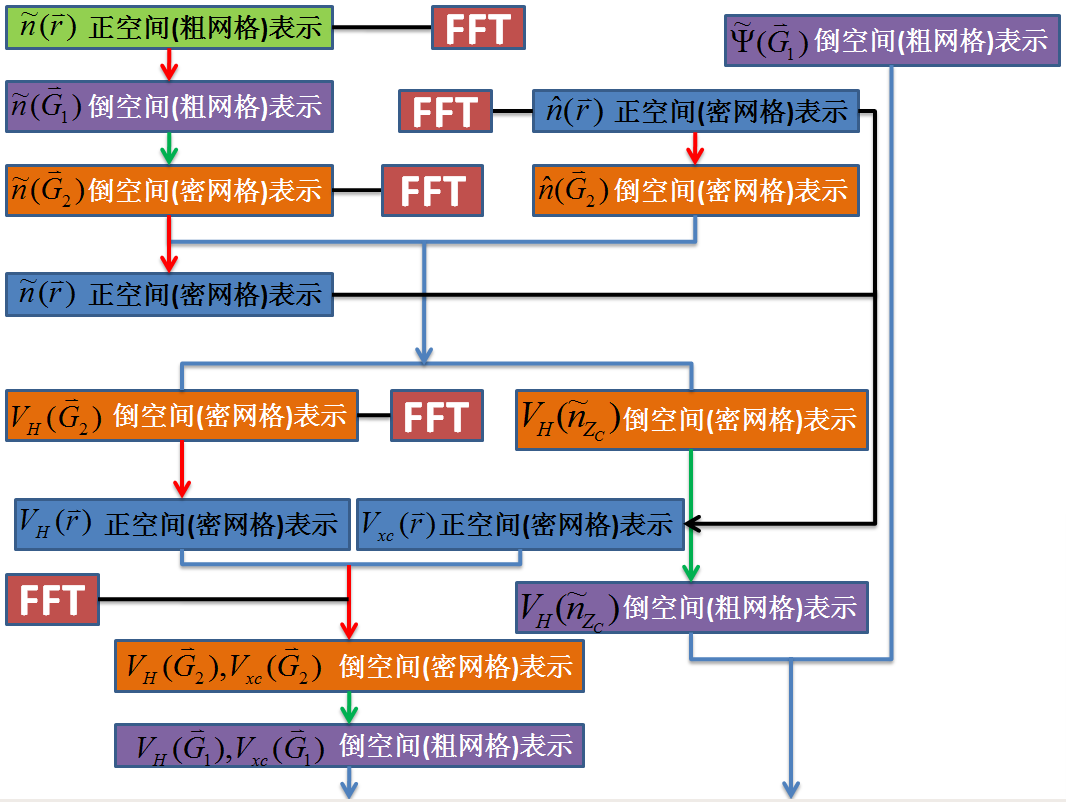
\includegraphics[height=2.7in,width=4.0in,viewport=0 0 800 600,clip]{Figures/dual_grid-2.png}
\caption{\tiny \textrm{The Schematic description of the dual grid technique.}}%(与文献\cite{EPJB33-47_2003}图1对比)
\label{PAW_dualgrid}
\end{figure} 
}

\frame
{
	\frametitle{一维\textrm{FFT}的\textrm{MPI}并行}
\begin{figure}[h!]
	\vspace{-0.15in}
\centering
%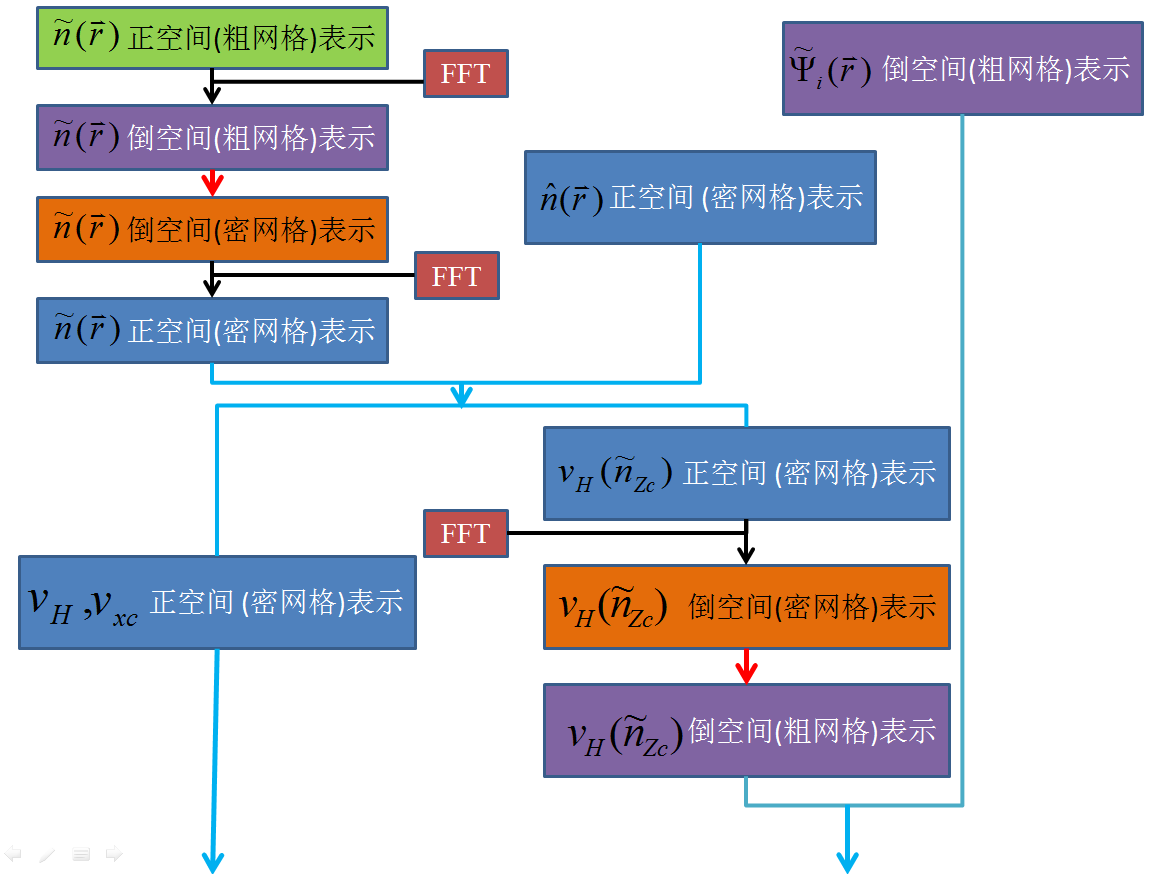
\includegraphics[height=2.7in,width=4.0in,viewport=0 0 1180 875,clip]{Figures/dual_grid.png}
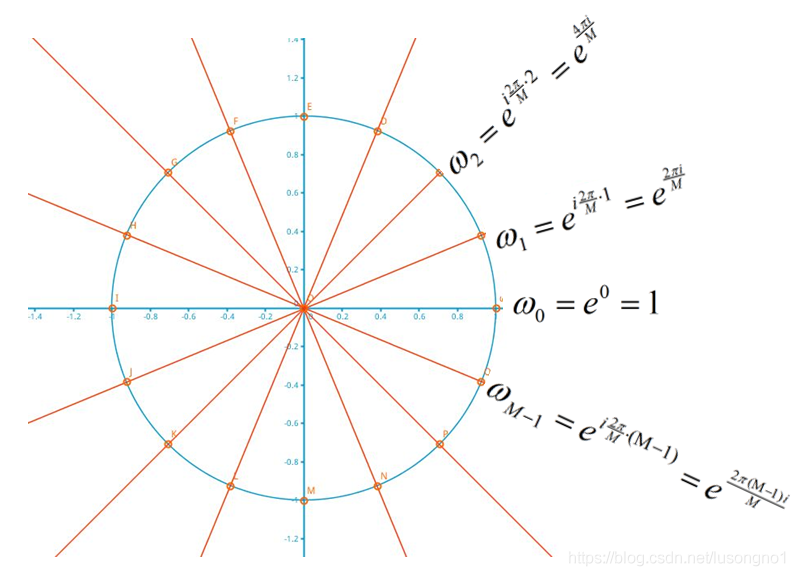
\includegraphics[height=1.55in,width=2.2in,viewport=0 10 810 580,clip]{Figures/FFT_para.png}
\vskip 0.5pt
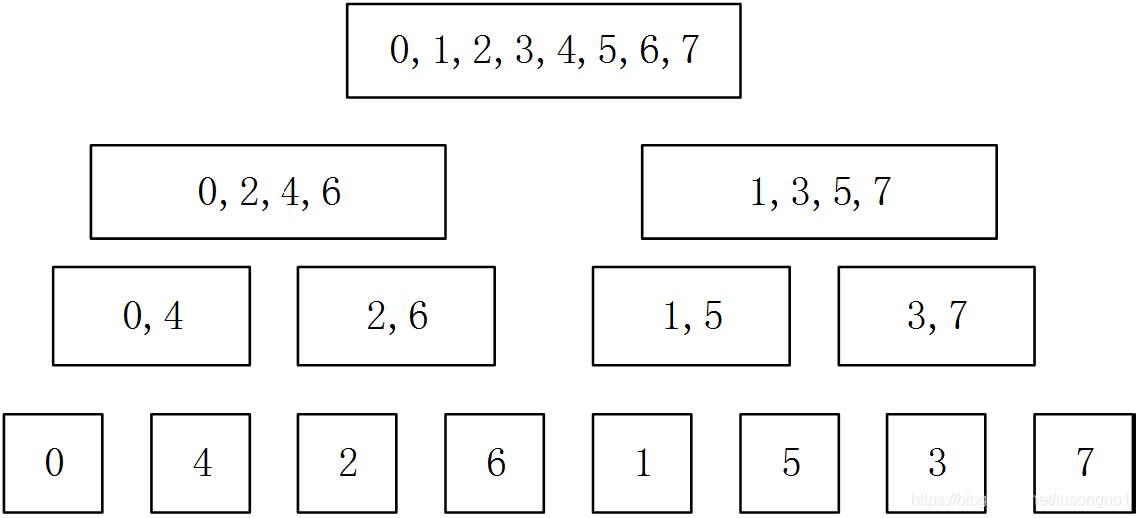
\includegraphics[height=1.2in,width=3.5in,viewport=0 0 1180 550,clip]{Figures/FFT_para-2.png}
\caption{\tiny \textrm{The Schematic description for FFT in MPI.}}%(与文献\cite{EPJB33-47_2003}图1对比)
\label{MPI-FFT}
\end{figure} 
}

\frame
{
	\frametitle{\textrm{VASP}计算的并行实现}
	\begin{itemize}
	     \item 中间层设计:~\textrm{FFT}网格、实空间基组与计算节点的匹配\\
		     \textcolor{magenta}{通过子程序\textrm{mgrid.F}生成中间层,实现并行负载与计算节点分配的匹配,减少\textrm{FFT}变换和实空间并行的节点间通信}
\begin{figure}[h!]
	\vspace{-0.25in}
\centering
%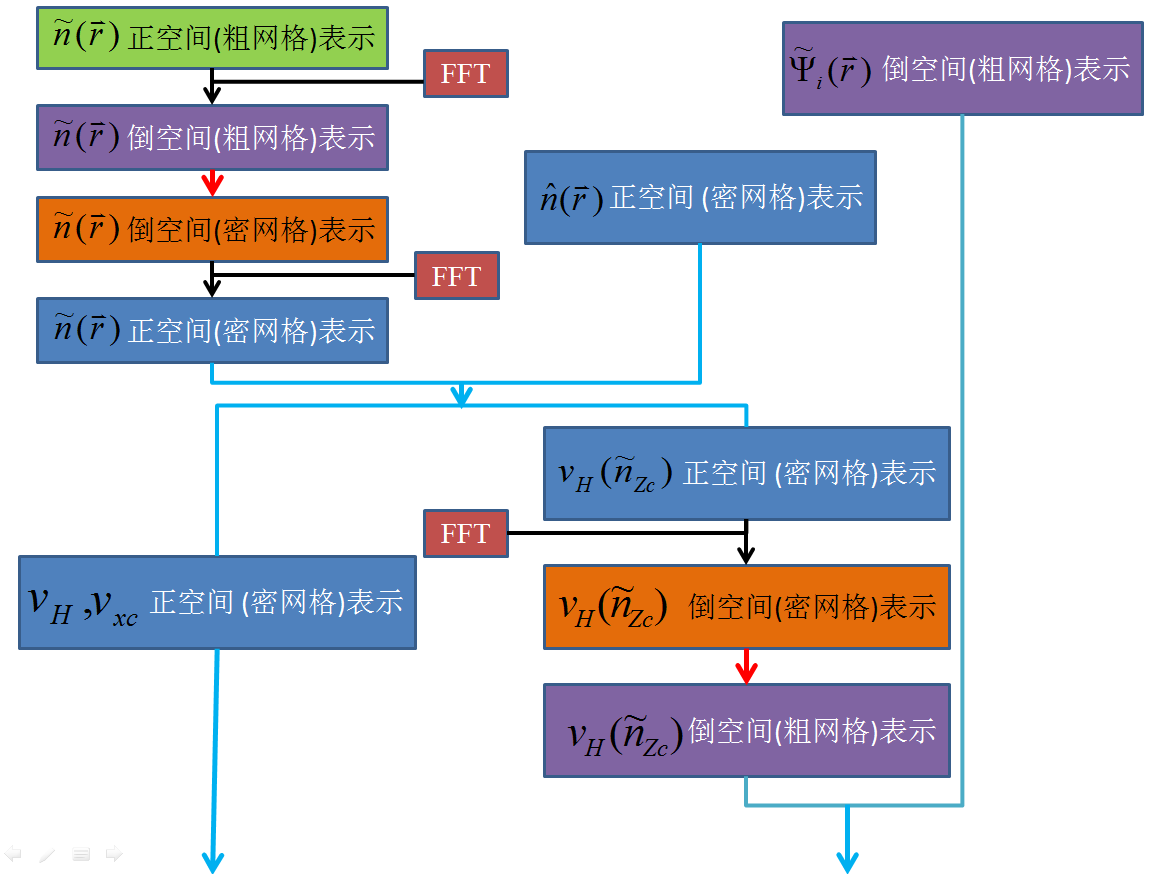
\includegraphics[height=2.7in,width=4.0in,viewport=0 0 1180 875,clip]{Figures/dual_grid.png}
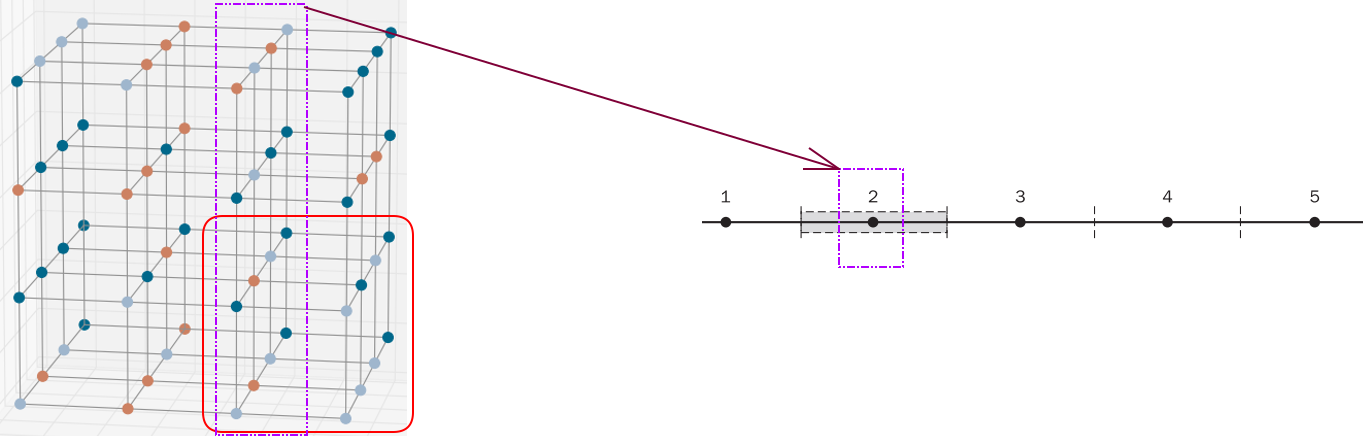
\includegraphics[height=1.0in,width=4.0in,viewport=0 0 1500 450,clip]{Figures/VASP_FFT-MPI_Reciprocal.png}
\vskip 0.5pt
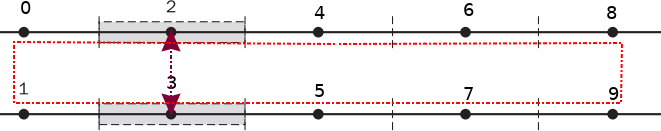
\includegraphics[height=0.7in,width=4.0in,viewport=0 0 730 150,clip]{Figures/VASP_FFT-MPI_Real.png}
\caption{\tiny \textrm{VASP:~ Reciprocal-Real space layout for grids in MPI.}}%(与文献\cite{EPJB33-47_2003}图1对比)
\label{MPI-FFT}
\end{figure} 
	\end{itemize}
}

\subsection{磁性与自旋波}
\frame
{
	\frametitle{自旋极化与磁振子}
	\begin{itemize}
		\item 凝聚态物质中,体系磁性态表现为长程的自旋磁矩有序状态
			\begin{enumerate}
				\item 由于电子-电子相互作用引起的原子局域磁矩(\textcolor{red}{自旋极化})
			\end{enumerate}
	\end{itemize}
		考虑自旋极化,单电子\textrm{Hamiltonian~}可写成二维矩阵
			\begin{displaymath}
				\hspace*{-10pt}\hat H=-\frac12\nabla^2+\sum_{jn}V_{\mathrm C}(|\vec r-\vec t_n-\vec a_j|)\mathbf{I}+\sum_{jn}U^{jn}\hat{V}_{\mathrm{ex}}(|\vec r-\vec t_n-\vec a_j|)(U^{jn})^{-1}
			\end{displaymath}
			矩阵$\mathbf{I}$是二维的单位矩阵,$V_{\mathrm{C}}\mathbf{I}$表示\textrm{Coulomb~}势\\
			矩阵$\mathbf{U}$表示空间坐标与局域坐标的变换关系,选定$z$-轴平行于磁场方向,用\textrm{Euler~}角表示为
			\begin{displaymath}
				\mathbf{U}=\left(
				\begin{matrix}
					\cos(\frac12\beta)\mathrm{exp}[-\mathrm{i}(\alpha+\gamma)/2] &-\sin(\frac12\beta)\mathrm{exp}[-\mathrm{i}(\alpha-\gamma)/2]\\
					\sin(\frac12\beta)\mathrm{exp}[\mathrm{i}(\alpha-\gamma)/2] &\cos(\frac12\beta)\mathrm{exp}[\mathrm{i}(\alpha+\gamma)/2]
				\end{matrix}\right)
			\end{displaymath}
		}

\frame
{
	\frametitle{自旋极化与磁振子}
			局域坐标下,交换势可以表示为
			\begin{displaymath}
				\hat{V}_{\mathrm{ex}}(r)=\left(
				\begin{matrix}
					V_{\mathrm{ex}}^+(r) &0\\
					0 &V_{\mathrm{ex}}^-(r)
				\end{matrix}\right)
			\end{displaymath}
	\begin{itemize}
		\item 局域磁矩间交换作用引起长程磁有序(\textcolor{red}{\textrm{Heisenberg~}}交换)
		\item 除了局域磁矩交换引起的磁有序结构,还有由于能带中巡游电子引起的磁性,称为能带磁性(或巡游电子磁性)
	\end{itemize}
	在能带理论中,磁有序态通过考虑自旋极化,引起\textrm{Hamiltonian~}的改变(\textrm{Zeeman}场强$H_{\mathrm{Zeeman}}$)引入:\\
	自旋极化磁矩$m=n^{\uparrow}-n^{\downarrow}$,引起的势能改变$V_m=\mu H_{\mathrm{Zeeman}}$
	\begin{displaymath}
		\begin{aligned}
			E=&E(V_m)\equiv E_{total}(V_m)\\
			m(\vec r)=&-\frac{\mathrm{d}E}{\mathrm{d}V_m(\vec r)}\\
			\chi(\vec r,\vec r^{\prime})=&-\frac{\mathrm{d}m(\vec r)}{\mathrm{d}V_m(\vec r^{\prime})}=\frac{\mathrm{d}^2E}{\mathrm{d}V_m(\vec r)\mathrm{d}V_m(\vec r^{\prime})}
		\end{aligned}
	\end{displaymath}
}

\frame
{
	\frametitle{\textrm{Heisenberg~}交换模型}
\begin{figure}[h!]
%	\vspace{-0.10in}
\centering
%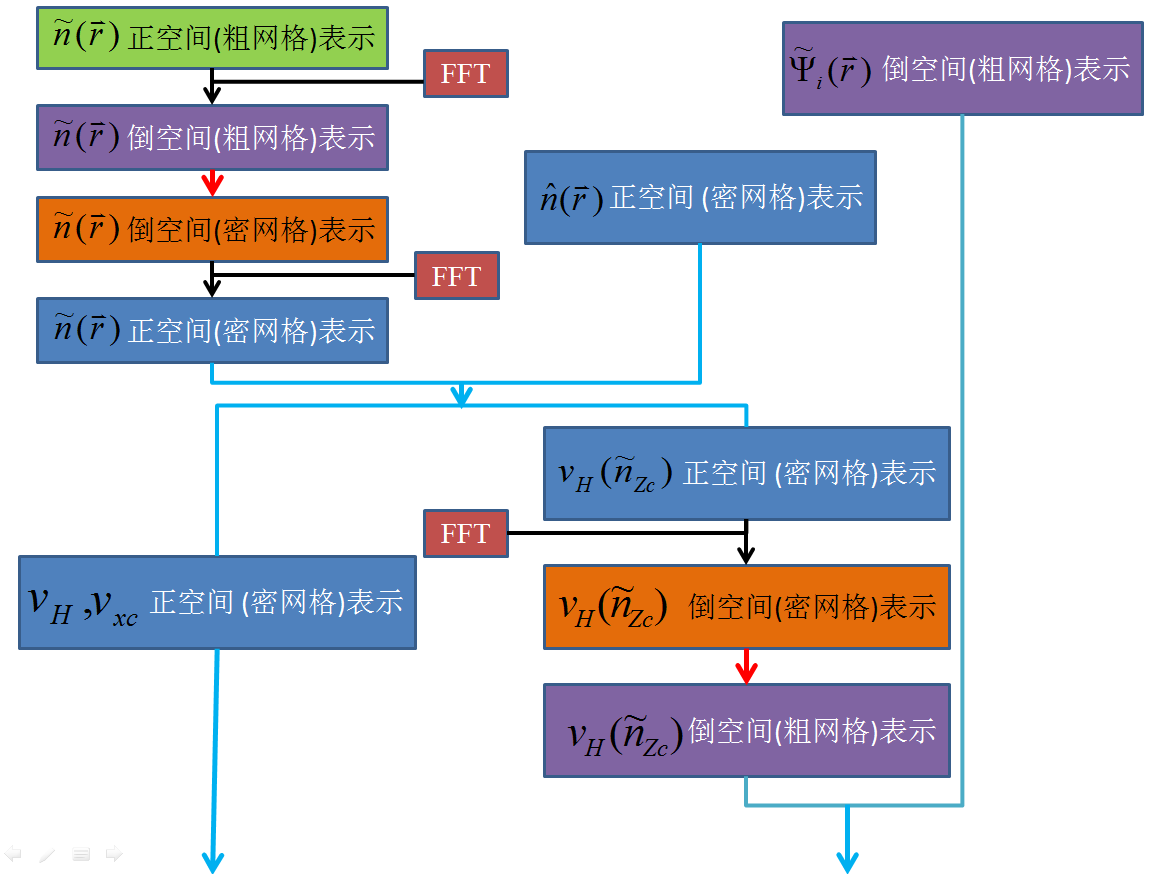
\includegraphics[height=2.7in,width=4.0in,viewport=0 0 1180 875,clip]{Figures/dual_grid.png}
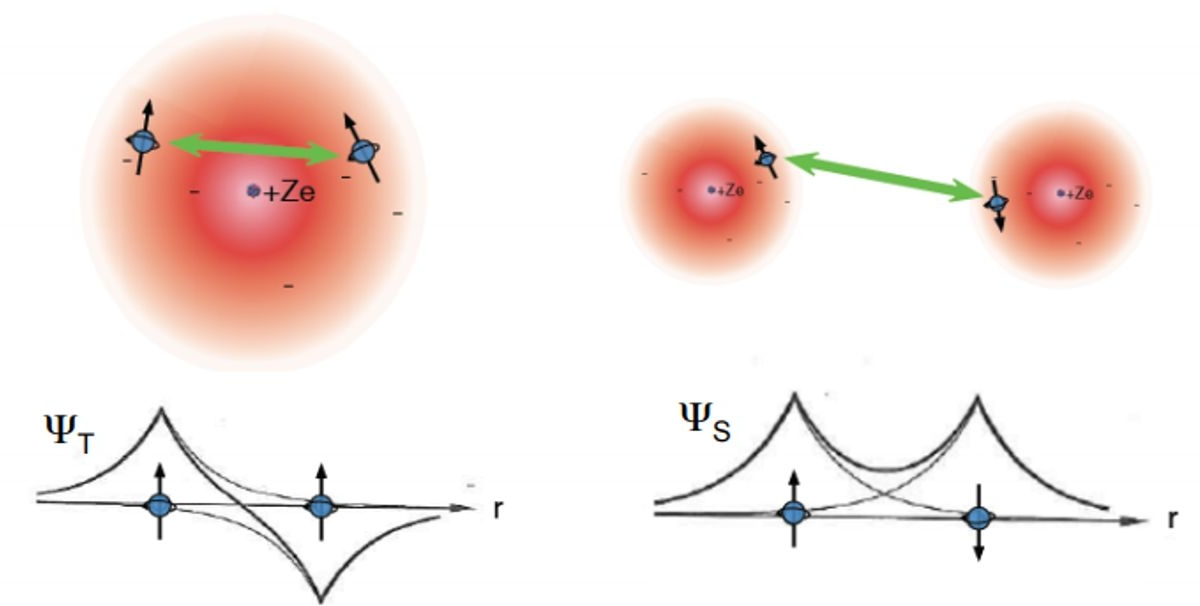
\includegraphics[height=2.0in,width=4.0in,viewport=0 0 580 290,clip]{Figures/Heisenberg_model.jpg}
\caption{\tiny \textrm{The model of Heisenberg-exchange coupling.}}%(与文献\cite{EPJB33-47_2003}图1对比)
\label{Heisenberg_Model}
\end{figure} 
}

\frame
{
	\frametitle{磁振子与自旋响应函数}
	\begin{itemize}
		\item 如果不考虑电子间相互作用,$E-\chi$曲线在净磁矩为0时有极小值,对应于自旋成对(抗磁态)
		\item 考虑电子交换作用,自旋有序(磁性态)能量更有利,因此$V_m(\vec r)$将依赖于$m(\vec r^{\prime})$:\\
			\begin{enumerate}
				\item 如果基态对应$\bar m>0$,则为铁磁态
				\item 如果基态对应$\bar m=0$,则为反铁磁态
			\end{enumerate}
		\item 平均场理论下,磁化率$\chi$即外加磁场的响应函数,\textrm{Stoner~}首先导出磁化率与电子态密度的关系
			\begin{displaymath}
				\chi=\frac{N(0)}{1-IN(0)}
			\end{displaymath}
			其中$N(0)$是\textrm{Fermi~}能级的态密度,磁化有关的有效外势$V_m=V_m^{ext}+Im$
	\end{itemize}
}

\frame
{
	\frametitle{铁磁、反铁磁和亚铁磁}
\begin{figure}[h!]
	\vspace{-0.20in}
\centering
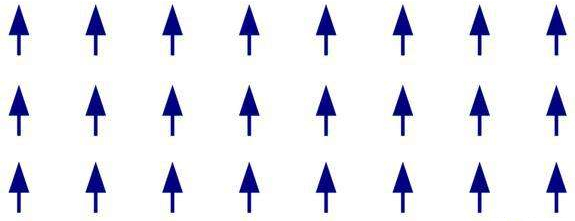
\includegraphics[height=0.95in,width=2.3in,viewport=0 0 350 230,clip]{Figures/Ferromagnetic.jpeg}\\
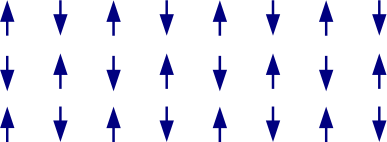
\includegraphics[height=0.85in,width=2.3in,viewport=0 -13 350 155,clip]{Figures/Antiferromagnetic.png}\\
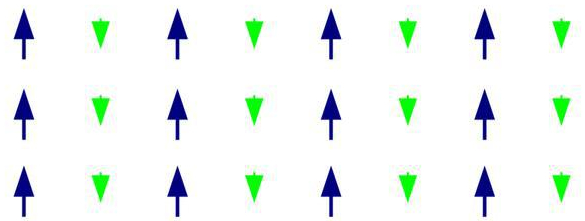
\includegraphics[height=0.88in,width=2.3in,viewport=0 0 350 225,clip]{Figures/Ferrimagnetic.jpeg}
\caption{\tiny \textrm{The model of Ferromagnetic, Antiferromagnetic and Ferrimagnetic.}}%(与文献\cite{EPJB33-47_2003}图1对比)
\label{Ferrimagneitic_Model}
\end{figure} 
}

\frame
{
	\frametitle{\textrm{Stoner}模型}
	\begin{itemize}
		\item \textrm{Stoner}将金属的磁性考虑为晶格中巡游的$3d$、$4s$\,电子贡献,其相互作用为$I$,\textrm{Fermi}面附近的\textrm{DOS}为$N(E_{\mathrm F})$
\begin{figure}[h!]
\centering
\vspace*{-0.05in}
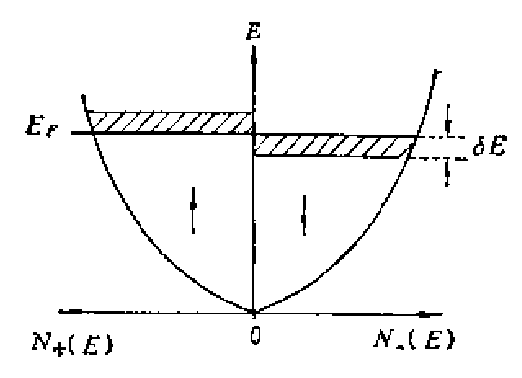
\includegraphics[height=1.0in,width=1.8in,viewport=0 0 800 380,clip]{Figures/Mag_Metal-T0.png}
\caption{\tiny \textrm{The Stoner model.}}%(与文献\cite{EPJB33-47_2003}图1对比)
\label{Mag_Metal-T0}
\end{figure}
		\item 体系的磁性由转变由\textrm{Fermi}面附近能量变化确定
			\begin{displaymath}
				\Delta E=N(E_{\mathrm F})\big[1-IN(E_{\mathrm F})\big](\delta E)^2
			\end{displaymath}
	\end{itemize}
}

\frame
{
	\frametitle{\textrm{Stoner}模型}
	\begin{itemize}
		\item \textrm{Stoner}模型中参数$I$\,主要反应$3d$电子的紧束缚特征,与晶体结构关系不大
		\item \textrm{Stoner}用于孤立原子体系,参数$I$描述自旋电子的裂分,要求:
			\begin{enumerate}
				\item \textcolor{blue}{对\textrm{LSDA}描述的单行列式态,参数$I$可以精确描述原子态的裂分}
				\item \textcolor{blue}{\textrm{LSDA}中应用\textrm{Stoner}模型,参数$I$\,与\textrm{Hubbard}规则的交换参数$U$一致}
			\end{enumerate}
		\item 参数$U$(或$I$~)、$J$的大小\\
			\begin{enumerate}
				\item \textcolor{red}{\textrm{Hund}规则的交换参数$J$的数量级:~ \textrm{1eV}
				\item \textrm{Hubbard}参数$U$的数量级:~\textrm{10eV}}
			\end{enumerate}
	\end{itemize}
}

\frame
{
	\frametitle{自旋波模型}
	\begin{itemize}
		\item 作为平均场近似,分子场理论成功描述了强磁性物质的自发磁化行为,但在低温和\textrm{Curie}温度附近,理论与实验存在明显偏差
		\item 自旋波理论是从体系\textcolor{red}{整体激发}的角度出发,解释自发磁化的低温行为
			\begin{enumerate}
				\item 0\textrm{K~}下电子自旋有序排列(系统基态)
\begin{figure}[h!]
\centering
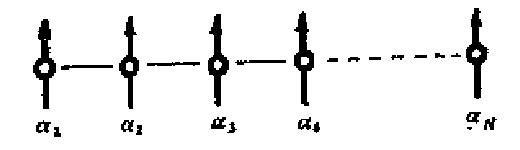
\includegraphics[height=0.50in,width=2.45in,viewport=10 10 600 150,clip]{Figures/Mag_spinwave-0.png}
\caption{\tiny \textrm{The ground state $|0\rangle$.}}%(与文献\cite{EPJB33-47_2003}图1对比)
\label{Mag_spinwave-0}
\end{figure}
				\item 温度略有升高时,电子自旋有一个发生翻转
\begin{figure}[h!]
\centering
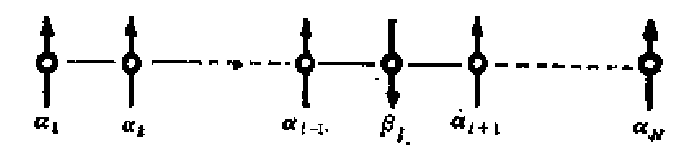
\includegraphics[height=0.50in,width=2.45in,viewport=10 10 680 150,clip]{Figures/Mag_spinwave-1.png}
\caption{\tiny \textrm{The spin flips at $l$:~ $|l\rangle$.}}%(与文献\cite{EPJB33-47_2003}图1对比)
\label{Mag_spinwave-1}
\end{figure}
			\end{enumerate}
	\end{itemize}
}

\frame
{
	\frametitle{自旋波模型}
	某个格点上出现自旋翻转,\textcolor{blue}{由于相邻格点间存在交换作用,使自旋趋于同向排列}
	\begin{itemize}
		\item \textcolor{red}{翻转的自旋将牵动临近格点自旋,使之趋于翻转}
		\item \textcolor{red}{近邻格点自旋力图驱使翻转的自旋重新翻转过来}
	\end{itemize}
	自旋的翻转不会停留在一个格点,而是以波的形式向周围传播:\\
	\textcolor{blue}{这种自旋翻转在晶体中的传播称为}\textcolor{red}{自旋波(又称磁激子)}
\begin{figure}[h!]
\centering
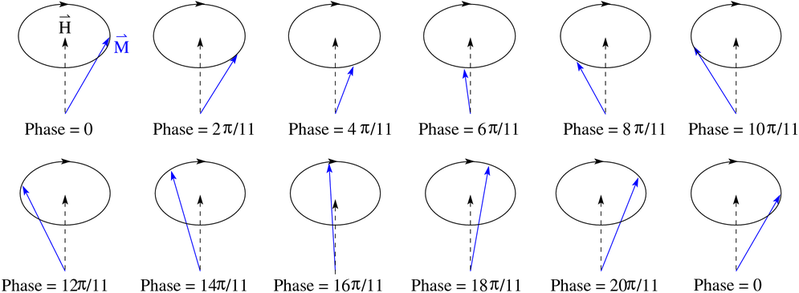
\includegraphics[height=1.15in,width=3.45in,viewport=0 0 830 300,clip]{Figures/Mag_spinwave-2.png}
\caption{\tiny \textrm{The schematic spin-wave.}}%(与文献\cite{EPJB33-47_2003}图1对比)
\label{Mag_spinwave-2}
\end{figure}
}

\frame
{
	\frametitle{非共线磁矩}
	\begin{itemize}
		\item 真实的物理体系中总会出现非共线的磁结构:\\\textcolor{blue}{特别是在铁磁/非磁金属界面上,铁磁性原子磁矩有可能形成非共线排列}
		\item 非共线体系中出现的新现象:\textcolor{blue}{电流诱导的自旋转矩}\\
			\textcolor{red}{非共线的原子磁矩与电子的自旋之间能够通过交换作用,进而引起电子在输运过程中发生自旋翻转,使得自旋向上和自旋向下的输运通道发生了混合}%,并且处在超导态的非磁金属还能够在铁磁体一侧诱导出长程的自旋三重态配对超导性}
		\item 由于非共线磁结构的引入使得问题变得复杂,目前的实验和理论还并不完备
	\end{itemize}
\begin{figure}[h!]
\centering
\vspace*{-0.10in}
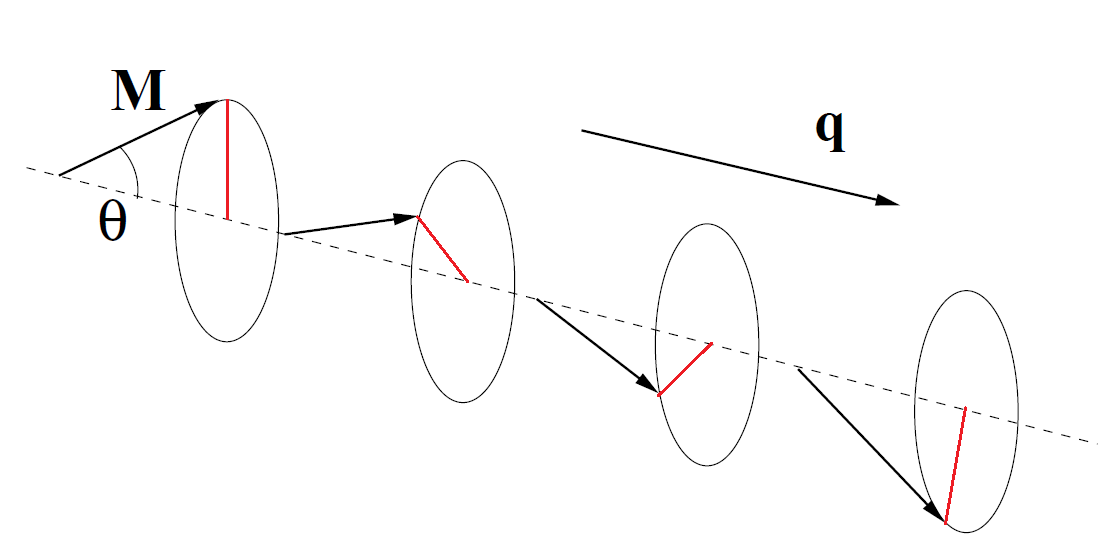
\includegraphics[height=1.05in,width=2.40in,viewport=10 10 840 370,clip]{Figures/Magnet_spinal_wave.png}
\caption{\tiny \textrm{The spiral magnetic structure.}}%(与文献\cite{EPJB33-47_2003}图1对比)
\label{Mag_spinal-wave}
\end{figure}
}

\frame
{
	\frametitle{\textrm{spin-spirals}}
	如果自旋方向随晶格周期也有周期性变化,这种自旋进动(\textrm{spin-spiral})引起体系具有额外的\textcolor{red}{自旋旋进周期性},因此自旋磁矩可以表示为
	\begin{displaymath}
		\vec m(\vec r+\vec R)=
		\begin{pmatrix}
			m_x(\vec r)\cos(\vec q\cdot\vec R)-m_y(\vec r)\sin(\vec q\cdot\vec R)\\
			m_x(\vec r)\sin(\vec q\cdot\vec R)+m_y(\vec r)\cos(\vec q\cdot\vec R)\\
			m_z(\vec r)
		\end{pmatrix}
	\end{displaymath}
	这里\textcolor{blue}{$\vec q$是倒空间中自旋进动的单位平移量},因此\\
	\textcolor{brown}{广义\textrm{Bl\"och}定理},波函数和\textrm{Hamiltonian}满足
	\begin{displaymath}
		\begin{aligned}
		&\begin{pmatrix}
			\Psi_{\vec k}^{\uparrow}(\vec r)\\
			\Psi_{\vec k}^{\downarrow}(\vec r)
		\end{pmatrix}=
		\begin{pmatrix}
			\mathrm{e}^{-\mathrm{i}\vec q\cdot\vec R/2} &0\\
			0 &\mathrm{e}^{+\mathrm{i}\vec q\cdot\vec R/2}
		\end{pmatrix}
		\begin{pmatrix}
			\Psi_{\vec k}^{\uparrow}(\vec r-\vec R)\\
			\Psi_{\vec k}^{\downarrow}(\vec r-\vec R)
		\end{pmatrix}\\
		&\begin{pmatrix}
			H^{\alpha\alpha}(\vec q) &V_{xc}^{\alpha\beta}\\
			V_{xc}^{\beta\beta} &H^{\beta\beta}(\vec q)
		\end{pmatrix}\rightarrow
		\begin{pmatrix}
			H^{\alpha\alpha}(\vec q) &V_{xc}^{\alpha\beta}\mathrm{e}^{-\mathrm{i}\vec q\cdot\vec r}\\
			V_{xc}^{\beta\alpha}\mathrm{e}^{+\mathrm{i}\vec q\cdot\vec r &H^{\beta\beta}(\vec q)}
		\end{pmatrix}
		\end{aligned}
	\end{displaymath}
}

\frame
{
	\frametitle{\textrm{DFT}框架下处理非共线磁矩}
	一般地,磁性体系下的\textrm{DFT~}的\textrm{Hamiltonian}:~
	\begin{displaymath}
		H=-\frac{\hbar^2}{2m}\nabla^2+V_{\mathrm{eff}}+\mu_B\vec\sigma\cdot\vec B_{\mathrm{eff}}
	\end{displaymath}
	这里$\mu_B\vec\sigma\cdot\vec B_{\mathrm{eff}}$表示\textcolor{blue}{自旋与有效磁场的相互作用}\\
	有效势、有效磁场是\underline{\textcolor{red}{外场}}和\underline{\textcolor{red}{交换-相关}势}、\underline{\textcolor{red}{交换-相关}场}之和
	\begin{displaymath}
		\begin{aligned}
			V_{\mathrm{eff}}=&V_{\mathrm{ext}}+V_{H}+V_{xc}\\
			\vec B_{\mathrm{eff}}=&\vec B_{\mathrm{ext}}+\vec B_{xc}
		\end{aligned}
	\end{displaymath}
	在\textrm{LDA}下,$E_{xc}(n,\vec m)=\int n\epsilon_{xc}(n,m)\mathrm{d}^3r$,因此交换-相互势和交换-相关场的表示
	\begin{displaymath}
		\begin{aligned}
			V_{xc}=&\frac{\partial E_{xc}(n,\vec m)}{\partial n}=&\epsilon_{xc}(n,m)+n\frac{\partial\epsilon_{xc}(n,m)}{\partial n}\\
			\vec B_{xc}=&\frac{\partial E_{xc}(n,\vec m)}{\partial\vec m}=&\frac{\partial\epsilon_{xc}(n,m)}{\partial m}\vec m
		\end{aligned}
	\end{displaymath}
}

\frame
{
	\frametitle{\textrm{DFT}框架下处理非共线磁矩}
\begin{itemize}
	\item 对\textrm{共线磁性},取外磁场方向与$\mathit{z}$轴方向一致
\begin{displaymath}
	\vec\sigma\cdot\vec B_{\mathrm{eff}}=\sigma_zB_{\mathrm{eff}}
\end{displaymath}
因为
\begin{displaymath}
	\sigma_z=\left(
	\begin{matrix}
		1 &0\\
		0 &-1
	\end{matrix}\right)
\end{displaymath}
由此可得
		\begin{displaymath}
			\hat V=V_{\mathrm{eff}}\mathbf{I}+B_{\mathrm{eff}}\sigma_z=\left(
			\begin{matrix}
				V_{\mathrm{eff}}+\mu_BB_{\mathrm{eff}} &0\\
				0 &V_{\mathrm{eff}}-\mu_BB_{\mathrm{eff}}
			\end{matrix}\right)
		\end{displaymath}
		这种情况下,\textcolor{red}{忽略旋-轨耦合\textrm{(SOC)},\textrm{spin-up}和\textrm{spin-dn}解耦}
\end{itemize}
}

\frame
{
	\frametitle{\textrm{DFT}框架下处理非共线磁矩}
\begin{itemize}
	\item 对\textrm{非共线磁性},标量点积$\mu_B\vec\sigma\cdot\vec B_{\mathrm{eff}}$必须考虑三个分量的贡献,注意到
\begin{displaymath}
	\sigma_x=\left(
	\begin{matrix}
		0 &1\\
		1 &0
	\end{matrix}\right)\quad
	\sigma_y=\left(
	\begin{matrix}
		0 &-\mathrm{i}\\
		\mathrm{i} &0
	\end{matrix}\right)
\end{displaymath}
由此可得
		\begin{displaymath}
			\hat V=V_{\mathrm{eff}}\mathbf{I}+\mu_BB_{\mathrm{eff}}\cdot\vec\sigma=\left(
			\begin{matrix}
				V_{\mathrm{eff}}+\mu_BB_z &\mu_B(B_x-\mathrm{i}B_y)\\
				\mu_B(B_x+\mathrm{i}B_y) &V_{\mathrm{eff}}-\mu_BB_z
			\end{matrix}\right)
		\end{displaymath}
		这种情况下,非对角元项将\textrm{spin-up}和\textrm{spin-dn}耦合在一起

\end{itemize}
}

\frame
{
	\frametitle{\textrm{VASP~}中一般非共线磁性态的计算}
	\textrm{J. K\"ubler}等指出\upcite{JAP63-3482_1988},根据密度泛函理论,当外势是矩阵元为$w^{\alpha\beta}(\vec r)$的$2\times2$矩阵时,令体系的密度矩阵为$\rho^{\alpha\beta}(\vec r)$,则\\
	\textcolor{blue}{体系的电荷密度可以表示为}
	\begin{displaymath}
		Tr[\rho^{\alpha\beta}(r)]\equiv n_{\mathrm{Tr}}(r)=\sum_{\alpha}n^{\alpha\alpha}(\vec r)
	\end{displaymath}
	因此总能量可以表示为
	
	\begin{displaymath}
		\begin{aligned}
			E[\rho^{\alpha\beta}]=&T_0+\sum_{\alpha\beta}\int w^{\alpha\beta}(\vec r)\rho^{\alpha\beta}(\vec r)\mathrm{d}^3r\\
			+&\iint\frac{n_{\mathrm{Tr}}(\vec r^{\prime})n_{\mathrm{Tr}}(\vec r)}{|\vec r-\vec r^{\prime}|}\mathrm{d}^3r\mathrm{d}^3r^{\prime}+E_{\mathrm{XC}}[\rho^{\alpha\beta}]
		\end{aligned}
	\end{displaymath}
}

\frame
{
	\frametitle{\textrm{VASP~}中一般非共线磁性态的计算}
	\textrm{D. Hobbs~}等\upcite{PRB62-11556_2000}\textcolor{red}{考虑磁化密度的贡献后,将总电荷密度矩阵表示为}
	\begin{displaymath}
		\rho^{\alpha\beta}(\vec r)=\left[n_{\mathrm{Tr}}(\vec r)\delta_{\alpha\beta}+\vec m(\vec r)\vec{\sigma}^{\alpha\beta}\right]/2
	\end{displaymath}
	\textcolor{blue}{磁化密度}的表示为
	\begin{displaymath}
		\vec m(\vec r)=\sum_{\alpha\beta}\rho^{\alpha\beta}(\vec r)\cdot\vec{\sigma}^{\alpha\beta}
	\end{displaymath}
	其中\textrm{Pauli~}自旋矩阵$\vec{\sigma}=(\sigma_x,\sigma_y,\sigma_z)$定义为
	\begin{displaymath}
		\sigma_x=\left( 
		\begin{matrix}
			0 &1\\
			1 &0
		\end{matrix}
		\right)\quad
		\sigma_y=\left( 
		\begin{matrix}
			0 &-\mathrm{i}\\
			\mathrm{i} &0
		\end{matrix}
		\right)\quad
		\sigma_z=\left( 
		\begin{matrix}
			1 &0\\
			0 &-1
		\end{matrix}
		\right)
	\end{displaymath}
	因此在\textrm{DFT}框架下能量密度泛函可以表示为
	\begin{displaymath}
		E=\sum_{\alpha}\sum_{n}f_n\langle\Psi_n^{\alpha}|-\frac12\nabla^2|\Psi_n^{\alpha}\rangle+E_{\mathrm{H}}[\textcolor{blue}{n_{\mathrm{Tr}}}+n_Z]+E_{\mathrm{XC}}[\textcolor{red}{\rho^{\alpha\beta}}]
	\end{displaymath}
}

\frame
{
	\frametitle{\textrm{VASP~}中一般非共线磁性态的计算}
	上述表达式中$f_n$是轨道占据数
	
	$E_{\mathrm{H}}[n_{\mathrm{Tr}}+n_Z]$是静电相互作用
	\begin{displaymath}
		E_{\mathrm{H}}[\textcolor{brown}{\rho}]=\frac12\iint\frac{\textcolor{brown}{\rho(\vec r)\rho(\vec r^{\prime})}}{|\vec r-\vec r^{\prime}|}\mathrm{d}\vec r\mathrm{d}\vec r^{\prime}
	\end{displaymath}
	这里$\textcolor{brown}{\rho}=n_{\mathrm{Tr}}+n_Z$

	在\textrm{LSDA}下,交换-相关能泛函表示为
	\begin{displaymath}
		\begin{aligned}
			E_{\mathrm{XC}}[\textcolor{red}{\rho^{\alpha\beta}}]=&\int\textcolor{blue}{n_{\mathrm{Tr}}(\vec r)}\epsilon_{\mathrm{XC}}[\textcolor{red}{\rho^{\alpha\beta}}]\mathrm{d}\vec r\\
			=&\int\textcolor{blue}{n_{\mathrm{Tr}}(\vec r)}\epsilon_{\mathrm{XC}}[\textcolor{blue}{n_{\mathrm{Tr}}(\vec r)},|\vec m(\vec r)|]\mathrm{d}\vec r
		\end{aligned}
	\end{displaymath}
}
%------------------------------------------------------------------------Reference----------------------------------------------------------------------------------------------
\frame[allowframebreaks]
{
\frametitle{主要参考文献}
{\tiny\textrm{
%\phantomsection\addcontentsline{toc}{section}{Bibliography}	 %直接调用\addcontentsline命令可能导致超链指向不准确,一般需要在之前调用一次\phantomsection命令加以修正	%
%\phantomsection\addcontentsline{toc}{section}{主要参考文献}	 %直接调用\addcontentsline命令可能导致超链指向不准确,一般需要在之前调用一次\phantomsection命令加以修正	%
\bibliography{Ref_2020-03-04}%
\bibliographystyle{../ref/mybib}%
}}
%\nocite{*}%
}

\section{复杂磁性结构与\rm{MagGene}软件}
\frame
{
	\frametitle{磁随机存储器\textrm{(MRAM)}}
磁性材料的核心问题:材料自旋磁结构的构筑、调控与设计
\begin{figure}[h!]
%\vspace*{-0.08in}
\centering
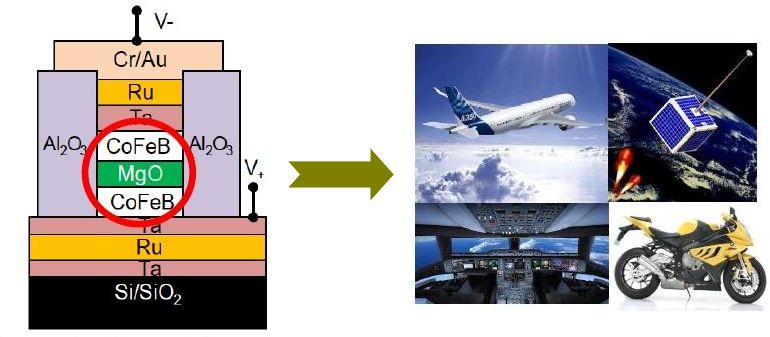
\includegraphics[height=1.85in,width=4.05in]{Figures/MRAM-Devices.png}
%\caption{\tiny \textrm{Simple Magnetic structure:~Ferromagnetism, Anti-Ferromagnetism, Ferrimagnetism}}%(与文献\cite{EPJB33-47_2003}图1对比)
\label{Fig:MRAM-Devices}
\end{figure}
}

\frame
{
	\frametitle{磁随机存储器\textrm{(MRAM)}}
	\begin{itemize}
		\item {\tiny \textrm{日本东北大学的科研团队成功开发出存储密度达128\textrm{Mb}的\textrm{STT-MRAM},写入速度达14\textrm{ns},可作为物联网和人工智能中用到的缓存使用}}
\begin{figure}[h!]
\vspace*{-0.08in}
\centering
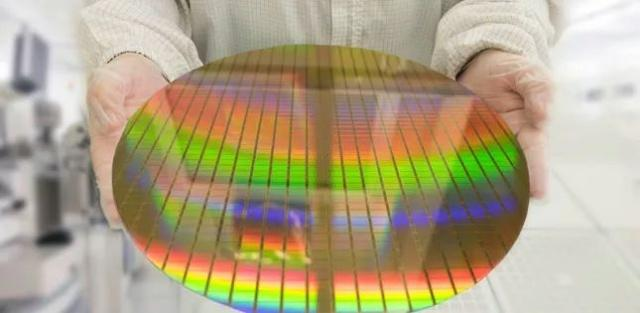
\includegraphics[height=1.00in,width=1.65in]{Figures/Si-crystal-Surface.png}
%\caption%(与文献\cite{EPJB33-47_2003}图1对比)
\label{Fig:Si-crystal-surface}
\end{figure}
\item {\tiny \textrm{韩国\textrm{Samsung}公司宣布已在一条基于28\textrm{nm~FD-SOI}工艺的生产线上,开始大规模生产和商业运输嵌入式\textrm{MRAM(eMRAM)}解决方案}}
\begin{figure}[h!]
\vspace*{-0.08in}
\centering
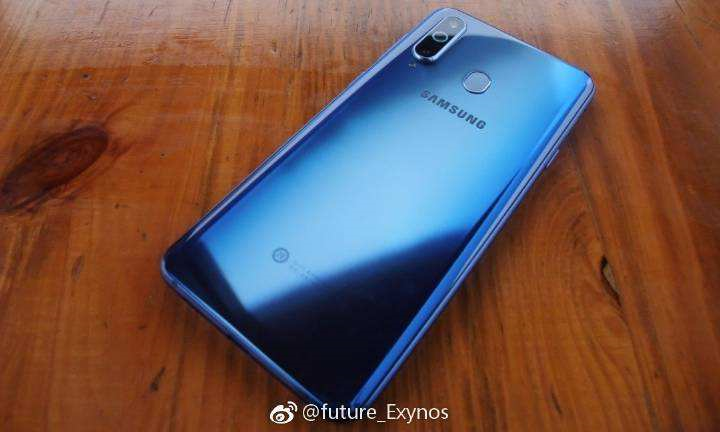
\includegraphics[height=1.00in,width=1.60in]{Figures/Samsung-cell.png}
%\caption%(与文献\cite{EPJB33-47_2003}图1对比)
\label{Fig:Samsung-cell}
\end{figure}
	\end{itemize}
}

\frame
{
	\frametitle{反铁磁存储}
	\begin{itemize}
		\item {\tiny \textrm{美国西北大学和意大利墨西拿大学的电气工程师们联合开发出一种新型的小巧但功能强大的存储设备,该设备使用创新的反铁磁\textrm{(AFM)}材料,而所需的耗电量之低创记录}}
\begin{figure}[h!]
\vspace*{-0.08in}
\centering
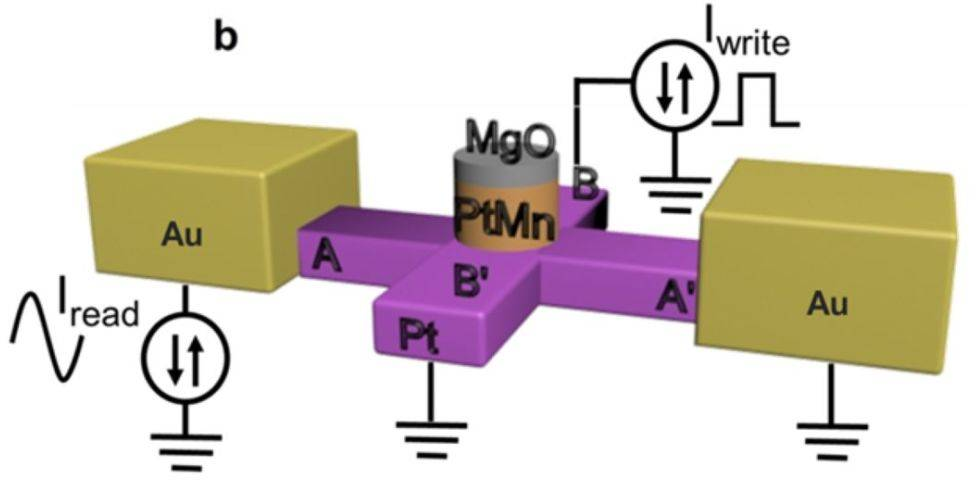
\includegraphics[height=0.95in,width=1.95in]{Figures/AFM-device.png}
%\caption{\tiny \textrm{}}%(与文献\cite{EPJB33-47_2003}图1对比)
\label{Fig:AFM-device}
\end{figure}
\item {\tiny \textrm{德国美因茨大学物理学家在反铁磁体中读出和写入信息,未来有望实现超高速、稳定的磁存储器}}
\begin{figure}[h!]
\vspace*{-0.04in}
\centering
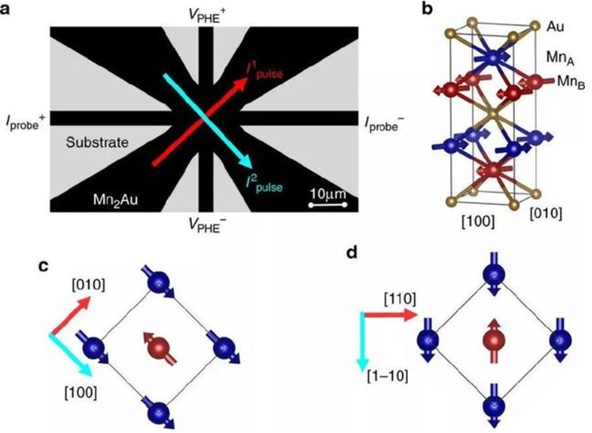
\includegraphics[height=1.05in,width=1.55in]{Figures/AFM-Memory.png}
%\caption{\tiny \textrm{}}%(与文献\cite{EPJB33-47_2003}图1对比)
\label{Fig:AFM-Memory}
\end{figure}
	\end{itemize}
}

\frame
{
	\frametitle{拓扑绝缘体}
	\begin{itemize}
		\item {\tiny \textrm{美国明尼苏达大学研究人员研究出一种涉及磁阻效应的新型拓扑绝缘体,有望应用于改善计算与存储}}
\begin{figure}[h!]
\vspace*{-0.04in}
\centering
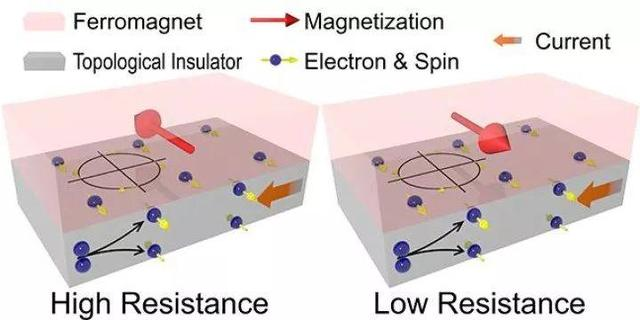
\includegraphics[height=0.95in,width=1.95in]{Figures/Topological-Insulator.png}
%\caption{\tiny \textrm{}}%(与文献\cite{EPJB33-47_2003}图1对比)
\label{Fig:Topological-Insulator}
\end{figure}
\item {\tiny \textrm{美国华盛顿大学研究人员采用仅有几个原子层厚度的二维磁性材料\ch{CrI3}来编码信息,有望实现更高密度的数据存储,并提高能量效率,从而革新计算技术和电子设备}}
\begin{figure}[h!]
\vspace*{-0.04in}
\centering
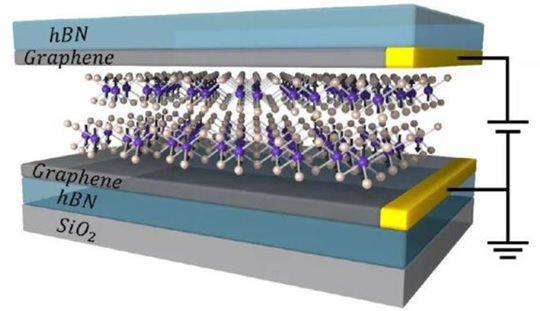
\includegraphics[height=1.05in,width=1.55in]{Figures/CrI3-Layer.png}
%\caption{\tiny \textrm{}}%(与文献\cite{EPJB33-47_2003}图1对比)
\label{Fig:CrI3-Layer}
\end{figure}
	\end{itemize}
}

\frame
{
	\frametitle{\textcolor{red}{开发\textrm{MRAM}技术瓶颈问题}}
	\begin{itemize}
		\item 如何构建一套具有范式意义的技术方法,使得我们能够\textcolor{red}{快速、精准地预测各类磁性材料的磁结构及磁参数}\\
			对加速开发\textrm{MRAM}具有至关重要的作用,目前属于国际空白
\begin{figure}[h!]
\vspace*{-0.04in}
\centering
\includegraphics[height=2.15in,width=3.25in]{Figures/Magnet-skyrmion.png}
%\caption{\tiny \textrm{}}%(与文献\cite{EPJB33-47_2003}图1对比)
\label{Fig:Magnet-skyrmion}
\end{figure}
	\end{itemize}
}

\subsection{复杂磁结构及其起源}
\frame
{
	\frametitle{简单磁结构~\textrm{.VS.}~复杂磁结构}
\begin{figure}[h!]
\vspace*{-0.08in}
\centering
\includegraphics[height=1.05in,width=0.75in]{Figures/Magnet-simple.png}
\caption{\tiny \textrm{Simple Magnetic structure:~Ferromagnetism, Anti-Ferromagnetism, Ferrimagnetism}}%(与文献\cite{EPJB33-47_2003}图1对比)
\label{Fig:Simple-Magnet}
\end{figure}
\begin{figure}[h!]
\vspace*{-0.08in}
\centering
\includegraphics[height=1.05in,width=2.35in]{Figures/Magnet-complex-compound.png}
\hskip 0.5pt
\includegraphics[height=1.05in,width=1.35in]{Figures/Magnet-complex.png}
\caption{\tiny \textrm{Complex Magnetic structure:~Spiral magnet, All-in-all-out, 3k-ordered}}%(与文献\cite{EPJB33-47_2003}图1对比)
\label{Fig:Simple-Magnet}
\end{figure}
}

\frame
{
	\frametitle{复杂磁结构的两大起源}
	\begin{itemize}
		\item 强磁阻挫:~\textrm{Kagome}晶格
\begin{figure}[h!]
\vspace*{-0.08in}
\centering
\includegraphics[height=0.7in,width=1.5in]{Figures/Magnet-Kagome-lattice.png}
\caption{\tiny \textrm{The Kagome lattice}}%(与文献\cite{EPJB33-47_2003}图1对比)
\label{Fig:Magnet-Kamoge}
\end{figure}
		\item 强自旋-轨道耦合:~稀土、锕系元素,核材料
\begin{figure}[h!]
\vspace*{-0.08in}
\centering
\includegraphics[height=0.85in,width=1.4in]{Figures/Magnet-Strong-SOC.png}
\includegraphics[height=0.85in,width=1.4in]{Figures/Nuclear-Power.png}
\caption{\tiny \textrm{Strong spin-orbit coupling and nuclear materials.}}%(与文献\cite{EPJB33-47_2003}图1对比)
\label{Fig:Magnet-SOC}
\end{figure}
	\end{itemize}
}

\subsection{遗传算法与结构预测}
\frame
{
	\frametitle{确定磁结构的方法和困难}
	\begin{itemize}
                \setlength{\itemsep}{5pt}
		\item \textcolor{blue}{确定磁结构的常用方法}
			\begin{enumerate}
                                \setlength{\itemsep}{3pt}
				\item 实验方法:~中子散射
				\item 理论方法:~人工猜测-计算验证方法
				\item 理论方法:~拟合磁自由度\textrm{Hamiltonian}-模拟退火
			\end{enumerate}
		\item \textcolor{blue}{复杂磁有序结构测定的困难}
			\begin{enumerate}
                                \setlength{\itemsep}{3pt}
				\item 中子散射:~某些实验材料质量欠佳、极端条件
				\item 人工猜想-计算验证方法:~效率低下,不适合复杂材料
				\item \textrm{Hamiltonian}-模拟退火:~\textrm{Hamiltonian}拟合困难,精度无法保证
			\end{enumerate}
			\textcolor{red}{本质的困难}:~海量潜在的可能结构导致常用方法失效
	\end{itemize}
}

\frame
{
	\frametitle{深度神经网络基础}
	\begin{itemize}
		\item 感知机(\textrm{Perceptron Learning Algorithm, PLA}):~最早的监督式训练算法,是神经网络构建的基础
\begin{figure}[h!]
\vspace*{-0.08in}
\centering
\includegraphics[height=0.50in]{Figures/DNN_PLA.png}
\caption{\tiny \textrm{Perceptron Learning Algorithm.}}%(与文献\cite{EPJB33-47_2003}图1对比)
\label{Fig:PLA}
\end{figure}
输出与输入之间将学习到一个线性关系,可有中间输出结果
\begin{displaymath}
	z=\sum_{i=1}^mw_ix_i+b
\end{displaymath}
中间结果连接一个神经元激活函数
\begin{displaymath}
	\mathrm{sign}(z)=\left\{
		\begin{aligned}
			-1\qquad &z<0\\
			1 \qquad &z\geqslant 0
		\end{aligned}\right.
\end{displaymath}
	\end{itemize}
}

\frame
{
	\frametitle{深度神经网络基础}
\begin{figure}[h!]
\vspace*{-0.08in}
\centering
\includegraphics[width=2.5in]{Figures/NN_PLA_example.png}
%\caption{\tiny \textrm{Perceptron Learning Algorithm.}}%(与文献\cite{EPJB33-47_2003}图1对比)
\label{Fig:PLA}
\end{figure}
在本例中,每一个输入数据都可以表示为一个向量$x = (x_1, x_2)$ ,而函数则是要实现“如果线以下,输出0;线以上,输出1”
}

\frame
{
	\frametitle{深度神经网络基础}
感知机模型只能用于二元分类,无法学习较为复杂的非线性模型,神经网络在感知机模型基础上作了扩展
\vskip 10pt
	\begin{itemize}
		\item 加入隐藏层(\textrm{hide layer}):~隐藏层可以有很多层,增强模型的表达能力
		\item 输出层的神经元可以有不止一个输出
		\item 对激活函数作扩展,如\textrm{Sigmoid}函数
			\begin{displaymath}
				f(z)=\dfrac1{1+\mathrm{e}^{-z}}
			\end{displaymath}
			其他的激活函数还有\textrm{tanx}、\textrm{softmax}和\textrm{ReLU}等
	\end{itemize}
}

\frame
{
	\frametitle{深度神经网络}
当前的深度神经网络~\textrm{(Deep Learning Neural Network)}~可以包含上百层神经元,通常有上万个参数,再加上超参数,实际的参数空间几乎是无限大的。如何从海量潜在的可能参数中做选择极具挑战性。
\begin{figure}[h!]
\vspace*{-0.08in}
\centering
\includegraphics[height=1.75in,width=3.75in]{Figures/ANN_Algorithm.png}
\caption{\tiny \textrm{Deep Learning Neural Network.}}%(与文献\cite{EPJB33-47_2003}图1对比)
\label{Fig:Deep-Learning-NN}
\end{figure}
}

\frame
{
	\frametitle{深度神经网络的前馈算法}
	以三层深度神经网络为例,说明深度神经网络的前馈算法
\begin{figure}[h!]
\vspace*{-0.08in}
\centering
\includegraphics[width=3.0in]{Figures/DNN_front_pro.jpg}
%\caption{\tiny \textrm{Perceptron Learning Algorithm.}}%(与文献\cite{EPJB33-47_2003}图1对比)
\label{Fig:PLA}
\end{figure}
}

\frame
{
	\frametitle{深度神经网络的前馈算法}
	假设激活函数为$\sigma(z)$,隐藏层和输出层的输出值为a,与感知机类似的思路,对于第二层的输出$a_1^2,a_2^2,a_3^2$,
	\begin{displaymath}
		\begin{matrix}
			a_1^2&=&\sigma(z_1^2)&=&\sigma(w_{11}^2x_1+w_{12}^2x_2+w_{13}^2x_3+b_1^2)\\
			a_2^2&=&\sigma(z_2^2)&=&\sigma(w_{21}^2x_1+w_{22}^2x_2+w_{23}^2x_3+b_2^2)\\
			a_3^2&=&\sigma(z_3^2)&=&\sigma(w_{31}^2x_1+w_{32}^2x_2+w_{33}^2x_3+b_3^2)
		\end{matrix}
	\end{displaymath}
	对于第三层的输出$a_1^3$,可有
	\begin{displaymath}
		a_1^3=\sigma(z_1^3)=\sigma(w_{11}^3a_1^2+w_{12}^3a_2^2+w_{13}^3a_3^2+b_1^3)
	\end{displaymath}
	一般地,假设第$l-1$层有$m$各神经元,则对于第$l$层的第$j$各神经元的输出$a_jl$可以表示为
	\begin{displaymath}
		a_j^l=\sigma(z_j^l)=\sigma(\sum_{k=1}^mw_{jk}^la_k^{l-1}+b_j^l)
	\end{displaymath}
	如果$l=2$,则$a_k^1$就是输入层$x_k$

	用矩阵表示
	\begin{displaymath}
		\vec a^l=\sigma(\vec z^l)=\sigma(\mathbf{W}^l\vec a^{l-1}+\vec b^l)
	\end{displaymath}
}

\frame
{
	\frametitle{遗传算法的基本原理}
	遗传算法\textrm{(Genetic Algorithm, GA)}是模拟生物进化论的自然选择和遗传学机理的计算模型,\textcolor{blue}{通过模拟自然进化过程搜索最优解}
	\begin{enumerate}
%		\item 优化问题可能潜在的解集构成一个种群(\textrm{population}),该种群由经过基因(\textrm{gene})编码的一定数目的个体(\textrm{individual})组成,每个个体是染色体(\textrm{chromosome})带有特征的实体
		\item 优化问题可能潜在的解集构成一个种群,该种群由经过基因编码的一定数目的个体组成,每个个体是带有一定的优化特征
%		\item 种群产生之后,借助于自然遗传学的遗传算子(\textrm{genetic operators})进行组合交叉(\textrm{crossover})和变异(\textrm{mutation}),产生新一代个体
		\item 种群产生之后,借助于自然遗传学的遗传算子进行组合交叉(\textrm{crossover})和变异(\textrm{mutation}),产生新一代个体
\begin{figure}[h!]
\vspace*{-0.10in}
\centering
\includegraphics[width=2.5in]{Figures/Genetic_Algorithm_basic.png}
%\caption{\tiny \textrm{Perceptron Learning Algorithm.}}%(与文献\cite{EPJB33-47_2003}图1对比)
\label{Fig:PLA}
\end{figure}
%		\item 按照适者生存和优胜劣汰的原理,在每一代,根据问题域中个体的适应度(\textrm{fitness}),选择(\textrm{selection})合适的个体,构成代表新的解集的种群
\vspace*{-0.10in}
		\item 按照适者生存和优胜劣汰的原理,在每一代,根据问题域中个体的适应度,选择合适的个体,构成代表新的解集的种群
%		\item 逐代(\textrm{generation})演化后,产生出越来越好的近似解(优化目标)
		\item 逐代演化后,产生出越来越好的近似解(优化目标)
	\end{enumerate}
}

\frame
{
	\frametitle{深度神经网络与遗传算法}
	\textcolor{blue}{深度神经网络类似问题的解决方案:~遗传算法}
\begin{minipage}[b]{0.49\textwidth}
\includegraphics[height=0.4in,width=2.08in,viewport=0 110 1280 350,clip]{Figures/Genetic_Algorithm-2.png}\\
\centering{\includegraphics[height=1.0in,width=1.08in,viewport=140 50 820 650,clip]{Figures/Genetic_Algorithm-1.png}}\\
\vskip 0.02pt
\includegraphics[height=0.7in,width=2.05in]{Figures/Genetic_Algorithm-3.png}\\
\centering{\textcolor{red}{\textrm{\tiny GACNN:~利用遗传算法训练深度卷积神经网络}}}
\end{minipage}
\hfill
\begin{minipage}[b]{0.49\textwidth}
\includegraphics[height=1.2in,width=1.9in]{Figures/Genetic_Algorithm-5.png}\\
\vskip 0.5pt
\includegraphics[height=0.55in,width=1.95in]{Figures/Genetic_Algorithm-4.png}\\
\centering{\textcolor{red}{\textrm{\tiny 多智能体强化学习:~神经网络}}}
\end{minipage}
}

\frame
{
	\frametitle{晶体结构优化的复杂性}
	\begin{itemize}
		\item \textcolor{blue}{晶体结构预测与搜索中也遇到类似问题}\\
		在已知元素种类的条件下,有可能预测或搜索材料晶体的结构;~但是材料的等能面存在无数个局域极小点,因而可能的晶体结构也是无限多的\\
		这使得晶体结构的预测与搜索极其困难
\begin{figure}[h!]
\centering
\includegraphics[height=1.3in,width=1.3in]{Figures/Struct-predict-3.png}
\hskip 1.0pt
\includegraphics[height=1.1in,width=2.25in]{Figures/Total_energy_opt.png}
\caption{\tiny \textrm{The structure of Perovskite and schematic for the energy minimum searching.}}%(与文献\cite{EPJB33-47_2003}图1对比)
\label{Fig:Structure-optimized}
\end{figure}
	\end{itemize}
}

\frame
{
	\frametitle{晶体结构优化问题的解决}
	\textcolor{blue}{解决方案:~遗传算法、粒子群方法等}
\begin{figure}[h!]
\centering
\includegraphics[height=1.0in,width=1.7in]{Figures/Struct-predict-1.png}
\includegraphics[height=1.0in,width=2.2in]{Figures/Struct-predict-2.png}
\vskip 8.0pt
\includegraphics[height=0.7in,width=2.2in]{Figures/Logo_USPEX.png}
\hskip 1.0pt
\includegraphics[height=1.0in,width=1.8in]{Figures/Logo_Calypso.png}
%\caption{\tiny \textrm{The structure of Perovskite and schematic for the energy minimum searching.}}%(与文献\cite{EPJB33-47_2003}图1对比)
\label{Fig:Structure-optimized-2}
\end{figure}
}

\frame
{
	\frametitle{磁结构遗传算法预测软件\textrm{MagGene}}
\begin{figure}[h!]
\centering
\includegraphics[height=2.5in,width=1.8in]{Figures/MagGene-copyright.png}
\hspace*{0.1in}
\includegraphics[height=2.5in,width=1.8in]{Figures/MagGene-Patent-inv.png}
%\caption{\tiny \textrm{The flow of MagGene.}}%(与文献\cite{EPJB33-47_2003}图1对比)
\label{Fig:MagGenea-Patent}
\end{figure}
}

\frame
{
	\frametitle{磁结构遗传算法预测软件\textrm{MagGene}}
鉴于遗传算法在深度学习和晶体结构预测中的成功应用,这种方法在磁结构预测中也大有用武之地。\textrm{MagGene}就是整合遗传算法和常用的第一性原理计算软件预测材料磁结构新型软件。
\begin{figure}[h!]
\centering
\includegraphics[height=2.2in,width=2.2in]{Figures/MagGene-Flow.png}
\caption{\tiny \textrm{The flow of MagGene.}}%(与文献\cite{EPJB33-47_2003}图1对比)
\label{Fig:MagGene-Flow}
\end{figure}
}

\frame
{
	\frametitle{磁结构计算中的一些处理}
	遗传算法预测磁结构过程中的多样性(\textrm{diversity})保持
	\begin{itemize}
		\item 磁结构搜索中的每一代都引入随机结构
		\item 放弃重复结构
			\begin{enumerate}
				\item \textcolor{magenta}{\textrm{collinear}}:\\
					通过对比产生每个新一代磁结构,去除重复结构
				\item \textcolor{magenta}{\textrm{noncollinear}}:\\
					引入磁结构相似度系数
					\begin{displaymath}
						s_{i,j}=\sqrt{\dfrac{\sum\limits_{n=1\atop t=x,y,z}^N(M_i^{n,t}-M_j^{n,t})^2}N}
					\end{displaymath}
					$M_i^{n,t}$表示第$i$种结构的第$n$个磁性原子的磁矩$t$分量\\
					当相似度系数大于某个指定的临界值\textcolor{magenta}{\textrm{similarity\_criteria}},则放弃相对稳定性低的结构
			\end{enumerate}
	\end{itemize}
}

\frame
{
	\frametitle{磁结构计算中的一些处理}
	由于磁相互作用一般都较弱,相比非磁性体系,磁性计算的收敛困难得多,难收敛体系的处理是控制磁结构搜索计算量的重要因素
	\begin{itemize}
		\item 经验表明:~真实基态一般不是难收敛结构
		\item 每一代的难收敛结构存在,会通过误差带\textrm{(error bar)},指向伪基态\textrm{(fake ground state)},导致磁结构搜索时间延长
		\item \textrm{MagGene}通过对难收敛结构的能量外加高的赝能量\textrm{(pseudo energy)},尽可能排除难收敛结构的干扰
	\end{itemize}

	\begin{displaymath}
		\mbox{\textcolor{blue}{\textrm{MagGene}}通过}\left\{
			\begin{aligned}
				&\mbox{\textcolor{magenta}{扩大搜索结构多样性}}\\
				&\mbox{\textcolor{magenta}{经验地消除伪基态}}
			\end{aligned}
			\right.
	\end{displaymath}
	\centering{有效地提高了磁结构搜索的效率和可靠性}
}

\frame
{
	\frametitle{\textrm{MagGene}的主要功能}
	\begin{itemize}
                \setlength{\itemsep}{15pt}
		\item \textcolor{blue}{\textrm{MagGene}的主要功能}:
			\begin{enumerate}
                                \setlength{\itemsep}{10pt}
				\item 自动产生可能的磁结构
				\item 自动生成第一性原理程序的输入文件
				\item 自动分析第一性原理程序的计算结果
				\item 筛选并优化磁结构,反复迭代,直至最终得到基态磁结构
			\end{enumerate}
		\item \textcolor{blue}{程序语言}:~\textrm{Fortran~95}
		\item \textcolor{blue}{第一原理计算程序}:~\textrm{VASP}
	\end{itemize}
}

\frame
{
	\frametitle{\textrm{MagGene}的主要文件}
	\begin{itemize}
		\item \textcolor{blue}{主输入文件:~\textrm{input.dat}}
\begin{figure}[h!]
	\vspace{-0.10in}
\centering
\includegraphics[height=1.0in,width=1.3in, viewport=0 20 400 290, clip]{Figures/MagGene-input.png}
%\caption{\tiny \textrm{The main input file for MagGene.}}%(与文献\cite{EPJB33-47_2003}图1对比)
\label{Fig:MagGene-input}
\end{figure}
\item \textcolor{blue}{第一性原理程序调用脚本:~\textrm{submit.sh}}
\begin{figure}[h!]
	\vspace{-0.08in}
\centering
\includegraphics[height=0.3in,width=1.8in, viewport=0 0 320 60, clip]{Figures/MagGene-submit-VASP.png}
%\caption{\tiny \textrm{The script for VASP in MagGene.}}%(与文献\cite{EPJB33-47_2003}图1对比)
\label{Fig:MagGene-script-VASP}
\end{figure}
\item \textcolor{blue}{第一原理程序输入文件:}\\
	\vspace{0.08in}
	\textcolor{magenta}{\textbf{INCAR, POSCAR, KPOINTS, POTCAR}}
	\end{itemize}
}

\frame[allowframebreaks]
{
	\frametitle{\textrm{MagGene}的主要输入参数}
	\begin{itemize}
                \setlength{\itemsep}{12pt}
		\item \textcolor{purple}{\textrm{noncollinear}}:~ 0~或~1;~指定是否在非共线磁有序中搜索基态
		\item \textcolor{purple}{\textrm{restart}}:~ 0~或~1;~指定当前计算是否是续算
		\item \textcolor{purple}{\textrm{m\_atom\_list}}:~ 整数序列;~指定哪些原子带有磁性
		\item \textcolor{purple}{\textrm{generation}}:~ 整数;~指定最大遗传算法代数
		\item \textcolor{purple}{\textrm{population}}:~ 整数;~指定一代中的结构数
		\item \textcolor{purple}{\textrm{similarity\_criteria}}: 实数;~指定两个结构是否相同的判定标准
		\item \textcolor{purple}{\textrm{pop\_best}}:~ 整数;~指定每代中保留的最佳结构数
		\item \textcolor{purple}{\textrm{n\_random}}:~ 整数;~在每代中随机生成的结构数
		\item \textcolor{purple}{ \textrm{n\_mutation}}:~ 整数;~在每代中引入的变异结构数
		\item \textcolor{purple}{\textrm{delta\_mutation}}:~ 整数;~变异程度
		\item \textcolor{purple}{\textrm{norm\_mag}}:~ 实数序列;~指定每个原子的磁矩大小
		\item \textcolor{purple}{\textrm{fixm}}:~ 一个或三个实数;~限定系统总磁矩大小
		\item \textcolor{purple}{\textrm{afm}}:~ 0或1;~是否进行反铁磁结构搜索
		\item \textcolor{purple}{\textrm{dft\_coverage}}:~ 0或1;~是否抛掉密度泛函计算中未收敛的结构
	\end{itemize}
}

\section{\rm{MagGene}应用算例}
\frame
{
	\frametitle{块体\textrm{\ch{FeSe}}}
	\textrm{\ch{FeSe}}具有非常复杂的磁有序结构
	\begin{itemize}
		\item 块体\textrm{\ch{FeSe}}:~具有超导电性$\mathrm{T_c}\sim8\mathrm{K}$
\begin{figure}[h!]
%\vspace*{-0.08in}
\centering
\includegraphics[height=1.6in,width=2.20in]{Figures/FeSe-Mag-Tc.png}
\caption{\tiny \textrm{The hysteresis loop of \ch{FeSe} (bulk-structure). }}%(与文献\cite{EPJB33-47_2003}图1对比)
\label{Fig:Mag-bulk-FeSe}
\end{figure}
\textrm{F-C. Hsu, \textit{et al}. PNAS \textbf{23}, 14262~(2008)}
	\end{itemize}
}

\frame
{
	\frametitle{单层\textrm{\ch{FeSe}}}
	\begin{itemize}
		\item 单层\textrm{\ch{FeSe}}具有更高的转变温度$\mathrm{T_c}\sim65\mathrm{K}$
\begin{figure}[h!]
\vspace*{-0.08in}
\centering
\includegraphics[height=1.5in,width=2.80in]{Figures/FeSe-single-Mag-Tc.png}
\caption{\tiny \textrm{The  $\mathrm{T_C}$ for the monolayer-structure \ch{FeSe}.}}%(与文献\cite{EPJB33-47_2003}图1对比)
\label{Fig:Mag-surface-FeSe}
\end{figure}
\textrm{S. He, \textit{et al}.  Nat. Mater. \textbf{12}, 605~(2013)}
	\end{itemize}
}

\frame
{
	\frametitle{\textrm{\ch{FeSe}}磁结构的预测}
	计算使用包含32个原子的超元胞\\
\begin{figure}[h!]
\vspace*{-0.08in}
\centering
\includegraphics[height=2.35in,width=1.45in]{Figures/FeSe-struct-1.png}
\hskip 0.2in
\includegraphics[height=1.40in,width=1.80in]{Figures/FeSe-struct-2.png}
\caption{\tiny \textrm{The monolayer- and bulk-structure of \ch{FeSe} for calculated. }}%(与文献\cite{EPJB33-47_2003}图1对比)
\label{Fig:FeSe-Structure}
\end{figure}
}

\frame
{
	\frametitle{\textrm{\ch{FeSe}}磁结构的预测}
	单层\textrm{\ch{FeSe}}在第四代找到了最稳定的磁结构\\
	块体\textrm{\ch{FeSe}}在第十代找到了最稳定的磁结构
\begin{figure}[h!]
\vspace*{-0.08in}
\centering
\includegraphics[height=1.25in,width=1.60in]{Figures/FeSe-Generation-1.png}
\hskip 0.5pt
\includegraphics[height=1.25in,width=1.60in]{Figures/FeSe-Generation-2.png}
%\caption{\tiny \textrm{The monolayer-structure of \ch{FeSe}. and $\mathrm{T_C}$. }}%(与文献\cite{EPJB33-47_2003}图1对比)
\label{Fig:FeSe-Generation}
\end{figure}
\centering
计算参数\textrm{input.data}文件设置:\\
\fbox{%
		\parbox{0.7\textwidth}{%

	\tiny{	\textrm{\textcolor{purple}{noncollinear}=0}:~ \#共线磁结构搜索\\
		\textrm{\textcolor{purple}{afm}=1}:~ \#搜索反铁磁结构\\
\textrm{\textcolor{purple}{generation}=30}:~ \#演化30代\\
\textrm{\textcolor{purple}{population}=30}:~ \#每一代计算30个结构\\
\textrm{\textcolor{purple}{pop\_best}=8}:~ \#保留8个最优结构\\
\textrm{\textcolor{purple}{n\_random}=10}:~ \#每一代包含10个随机结构 }}
}
}

\frame
{
	\frametitle{单层\textrm{\ch{CrI3}}}
	\begin{itemize}
		\item 单层\textrm{\ch{CrI3}}在不同条件下具有不同的磁结构
\begin{figure}[h!]
\vspace*{-0.08in}
\centering
\includegraphics[height=1.85in,width=1.45in]{Figures/CrI3-magnet-struct-1.png}
\caption{\tiny \textrm{The different magnetic structure of monolayer-structure \ch{FeSe}.}}%(与文献\cite{EPJB33-47_2003}图1对比)
\label{Fig:Mono-layere-CrI3}
\end{figure}
\textrm{F. Zheng, \textit{et al}.  Nanoscale. \textbf{10}, 14298~(2018)}
	\end{itemize}
}

\frame
{
	\frametitle{单层\textrm{\ch{CrI3}}}
	\begin{itemize}
		\item \textrm{\ch{CrI3}}层间也有复杂的磁耦合行为
\begin{figure}[h!]
\vspace*{-0.08in}
\centering
\includegraphics[height=1.85in,width=2.05in]{Figures/CrI3-magnet-struct-2.png}
\caption{\tiny \textrm{The inter-layer magnet-coupling of \ch{FeSe}.}}%(与文献\cite{EPJB33-47_2003}图1对比)
\label{Fig:Inter-layer-CrI3}
\end{figure}
\textrm{B. Huang, \textit{et al}.  Nat. Nanotech. \textbf{13}, 544~(2018)}
	\end{itemize}
}

\frame
{
	\frametitle{单层\textrm{\ch{CrI3}}磁结构的预测}
	晶格常数为6.3\textrm{\AA}、7\textrm{\AA}和8\textrm{\AA}的单层\textrm{\ch{CrI3}}在第21、6和10代找到了最稳定的磁结构,分别是面内反铁磁、面外铁磁和面内铁磁。
\begin{figure}[h!]
\vspace*{-0.08in}
\centering
\includegraphics[height=1.15in,width=1.45in]{Figures/CrI3-struct.png}\\
\includegraphics[height=1.00in,width=1.22in]{Figures/CrI3-Generation-6.png}
\hskip 0.5pt
\includegraphics[height=1.00in,width=1.22in]{Figures/CrI3-Generation-7.png}
\hskip 0.5pt
\includegraphics[height=1.00in,width=1.22in]{Figures/CrI3-Generation-8.png}
\caption{\tiny \textrm{Atomic structure of \ch{CrI3} single layer and the MagGene calculation results for single layer with lattice parameters 6.3\AA, 7.0\AA, and 8.0\AA respectively.}}%(与文献\cite{EPJB33-47_2003}图1对比)
\label{Fig:FeSe-Generation}
\end{figure}
}

\frame
{
	\frametitle{单层\textrm{\ch{CrI3}}磁结构的预测}
\centering
计算参数\textrm{input.data}文件设置:\\
\vskip 0.3in
\fbox{%
		\parbox{0.7\textwidth}{%

		\textrm{\textcolor{purple}{noncollinear}=1}:~ \#非共线磁结构搜索\\
		\textrm{\textcolor{purple}{afm}=0}:~ \#不限于搜索反铁磁结构\\
\textrm{\textcolor{purple}{generation}=30}:~ \#演化30代\\
\textrm{\textcolor{purple}{population}=30}:~ \#每一代计算30个结构\\
\textrm{\textcolor{purple}{pop\_best}=8}:~ \#保留8个最优结构\\
\textrm{\textcolor{purple}{n\_random}=10}:~ \#每一代包含10个随机结构 }}
}

\frame
{
	\frametitle{\textrm{\ch{UO2}}晶体}
	\begin{itemize}
		\item \textrm{\ch{UO2}}具有非常复杂的磁有序结构
\begin{figure}[h!]
\vspace*{-0.08in}
\centering
\includegraphics[height=1.85in,width=3.25in]{Figures/UO2-complex-struct.png}
\caption{\tiny \textrm{The complexed magnetic-ordered structure of \ch{UO2}.}}%(与文献\cite{EPJB33-47_2003}图1对比)
\label{Fig:Inter-layer-CrI3}
\end{figure}
\textrm{J. T. Pegg, \textit{et al}.  Phys. Chem. Chem. Phys. \textbf{21}, 760~(2019)}
	\end{itemize}
}

\frame
{
	\frametitle{\textrm{\ch{UO2}}磁结构的预测}
	计算程序在第13代演化中找到\textrm{\ch{UO2}}正确的磁结构:~\textrm{3k}反铁磁
\begin{figure}[h!]
\vspace*{-0.08in}
\centering
\includegraphics[height=1.45in,width=1.20in]{Figures/UO2-struct.png}
\hskip 0.5pt
\includegraphics[height=1.45in,width=1.50in]{Figures/UO2-Generation.png}
%\caption{\tiny \textrm{The monolayer-structure of \ch{FeSe}. and $\mathrm{T_C}$. }}%(与文献\cite{EPJB33-47_2003}图1对比)
\label{Fig:FeSe-Generation}
\end{figure}
\textcolor{red}{\tiny{计算中使用了描述关联性之更好的\textrm{Meta-GGA}泛函\textrm{SCAN}来研究\textrm{\ch{UO2}}}}\\
\vskip 0.08in
\centering
计算参数\textrm{input.data}文件设置:\\
\fbox{%
		\parbox{0.7\textwidth}{%

	\tiny{	\textrm{\textcolor{purple}{noncollinear}=1}:~ \#非共线磁结构搜索\\
		\textrm{\textcolor{purple}{afm}=1}:~ \#搜索反铁磁结构\\
\textrm{\textcolor{purple}{generation}=30}:~ \#演化30代\\
\textrm{\textcolor{purple}{population}=30}:~ \#每一代计算30个结构\\
\textrm{\textcolor{purple}{pop\_best}=8}:~ \#保留8个最优结构\\
\textrm{\textcolor{purple}{n\_random}=3}:~ \#每一代包含3个随机结构 }}
}
}
%-----------------------------------------------------------------------------------------------------------------------------------------------------------------------%
\appendix
\frame
{
	\frametitle{\textrm{\ch{FeSe}}磁结构的预测:~\textrm{INCAR}}
\begin{figure}[h!]
\vspace*{-0.11in}
\centering
\includegraphics[height=2.85in,width=1.20in]{Figures/MagGene-FeSe-monolayer-INCAR.png}
\hskip 0.3in
\includegraphics[height=2.85in,width=1.20in]{Figures/MagGene-FeSe-bulk-INCAR.png}
%\caption{\tiny \textrm{The monolayer-structure of \ch{FeSe}. and $\mathrm{T_C}$. }}%(与文献\cite{EPJB33-47_2003}图1对比)
\label{Fig:FeSe-INCAR}
\end{figure}
}

\frame
{
	\frametitle{\textrm{\ch{CrI3}}磁结构的预测:~\textrm{INCAR}}
\begin{figure}[h!]
\vspace*{-0.11in}
\centering
\includegraphics[height=2.85in,width=1.20in]{Figures/MagGene-CrI3-6.3-INCAR.png}
\hskip 0.3in
\includegraphics[height=2.85in,width=1.20in]{Figures/MagGene-CrI3-7.0-INCAR.png}
%\caption{\tiny \textrm{The monolayer-structure of \ch{FeSe}. and $\mathrm{T_C}$. }}%(与文献\cite{EPJB33-47_2003}图1对比)
\label{Fig:CrI3-INCAR}
\end{figure}
}

\frame
{
	\frametitle{\textrm{\ch{UO2}}磁结构的预测:~\textrm{INCAR}}
\begin{figure}[h!]
\vspace*{-0.20in}
\centering
\includegraphics[height=3.00in,width=0.80in]{Figures/MagGene-UO2-INCAR.png}
%\caption{\tiny \textrm{The monolayer-structure of \ch{FeSe}. and $\mathrm{T_C}$. }}%(与文献\cite{EPJB33-47_2003}图1对比)
\label{Fig:UO2-INCAR}
\end{figure}
}

\frame
{
	\frametitle{\textrm{\ch{MnBiTe}}基态磁结构的预测}
\begin{figure}[h!]
\vspace*{-0.4in}
\centering
\includegraphics[height=2.00in,width=4.10in]{Figures/MagGene-MnBiTe.png}
%\caption{\tiny \textrm{The monolayer-structure of \ch{FeSe}. and $\mathrm{T_C}$. }}%(与文献\cite{EPJB33-47_2003}图1对比)
\label{Fig:MnBiTe}
\end{figure}
\begin{minipage}[!t]{0.49\textwidth}
 \vspace*{-35pt}
{\fontsize{7.5pt}{6.0pt}\selectfont{
	易磁化轴指向最近邻\textrm{\ch{Te}}的反铁磁基态\\
计算框架:~标准\textrm{DFT}+\textrm{SOC}(\textrm{PBE}泛函)}}
\end{minipage}
\begin{minipage}[b]{0.49\textwidth}
 \vspace*{-5pt}
{\fontsize{7.5pt}{6.0pt}\selectfont{
	易磁化轴沿着$z$方向的铁磁基态\\
	计算框架:~标准\textrm{DFT}+$U$($U$=3~\textrm{eV for }\textrm{\ch{Mn}}-$d$)+\textrm{SOC}(\textrm{PBE}泛函)}}
\end{minipage}
\vskip 5pt
考虑了\textrm{Hubbard}+$U$修正电子相关效应的计算框架下得到的基态磁结构与实验相符
}
%------------------------------------------------------------------------------------------------------------------------------------------------------------------------------%
%\frame
%{
%\frametitle{主要参考文献}
%\begin{thebibliography}{99}
%{\small
%\bibitem{Singh_Book}\textrm{D. J. Singh. \textit{Plane Wave, PseudoPotential and the LAPW method} (Kluwer Academic, Boston,USA, 1994)}					%
%\end{thebibliography}
%  \nocite{*}																				%
%}
%}

%-------------------------------------------------------------------------Thanks------------------------------------------------------------------------------------------------
%\section{致谢}
%\frame
%{
%\frametitle{致$\quad$谢}
%\begin{itemize}
%    \setlength{\itemsep}{20pt}
%  \item 感谢本团队高兴誉、吴泉生、宋红州等各位老师参与的讨论
%  \item 感谢莫所长、宋主任以及软件中心各位老师和同事
%  \item 感谢王崇愚先生的帮助
%\end{itemize}
%}

\logo{}									%不显示logo
\frame
{
\vskip 60 pt
%\hskip 10pt \textcolor{blue}{\Huge 感谢答辩委员会各位老师\,\textrm{!}}\\
\vskip 35 pt
\hskip 60pt \textcolor{blue}{\Huge 谢谢大家\:!}
%\vskip 15 pt
%\hskip 40pt \textcolor{blue}{\Huge \textrm{for your attention\:!}}
}

%\frame
%{
%\begin{figure}[h!]
%\centering
%\animategraphics[autoplay, loop, height=2.1in]{1}{Figures/Prof_Liu-}{06}{11}
%\label{Prof_Liu}
%\end{figure}
%}
%
%-------------------------------------------------------------------------------------------------------------------------------------------------------------------------------

\clearpage
%\end{CJK*}
\end{document}
